% =====================================================================
% Archivo: AreasdeOportunidadCEL.tex
% Propósito: Documento "Áreas de Oportunidad del Sistema CEL"
% Estilo: Español institucional (México) con clase cel.cls
% Integración: Guía horizontal y mejores prácticas SENER
% =====================================================================

\documentclass{cel}

% --- Metadatos del Documento ---
\title{Áreas de Oportunidad del Sistema de Certificados de Energía Limpia (CEL)}
\subtitle{Análisis Integral y Propuestas de Modernización}
\author{SENER}
\date{\today}
\institucion{Secretaría de Energía (SENER)}
\unidad{Unidad de Planeación Energética}
\setDocumentoCorto{Áreas CEL}
\palabrasclave{Energía, CEL, Certificados, Modernización}
\version{1.0}

% --- Metadatos PDF/UA (Accesibilidad Universal) ---
\hypersetup{
  pdftitle={Áreas de Oportunidad del Sistema de Certificados de Energía Limpia (CEL)},
  pdfauthor={SENER},
  pdfsubject={Sistema CEL - Áreas de Oportunidad},
  pdfkeywords={Energía, CEL, Certificados, Modernización, Sistema},
  pdfversion={1}
}

\begin{document}

% Portada institucional con fondo personalizado
\portadafondo[img/portada.png]

% Página de créditos/directorio
\paginacreditos{
\begin{center}
{\Large\bfseries\color{gobmxGuinda} Directorio}\\[1cm]
\end{center}

\vspace{1cm}

\begin{center}
{\large\bfseries\color{senerGuindaOscuro} Secretaría de Energía}\\[0.5cm]
{\normalsize Luz Elena González Escobar}\\
{\small\color{gobmxGris} Secretaria de Energía}\\[1cm]

{\large\bfseries\color{senerGuindaOscuro} Unidad de Planeación Energética}\\[0.5cm]
{\normalsize Dr. Leonardo Beltrán Rodríguez}\\
{\small\color{gobmxGris} Titular de la Unidad de Planeación Energética}\\[1cm]

{\large\bfseries\color{senerGuindaOscuro} Comisión Nacional de Energía}\\[0.5cm]
{\normalsize Ing. Arturo Herrera Gutiérrez}\\
{\small\color{gobmxGris} Comisionado Presidente}\\[1cm]

{\large\bfseries\color{senerGuindaOscuro} Equipo Técnico}\\[0.5cm]
{\normalsize Dirección General de Planeación e Información Energéticas}\\
{\normalsize Dirección General de Electricidad}\\
{\normalsize Dirección de Energías Limpias}\\
\end{center}
}

% Índice General (TOC)
{
  \hypersetup{linkcolor=gobmxGuinda}
  \tableofcontents
}
\newpage

% =====================================================================
% INTRODUCCIÓN
% =====================================================================
\phantomsection
\addcontentsline{toc}{section}{Introducción}
\section*{Introducción}

El Sistema de Certificados de Energía Limpia (S-CEL) constituye uno de los instrumentos centrales de la política de transición energética de México. Establecido en el marco de la Ley del Sector Eléctrico y operado mediante las Disposiciones Administrativas de Carácter General emitidas por la Comisión Nacional de Energía (CNE), este sistema busca incentivar la generación de energía limpia y garantizar el cumplimiento de las metas nacionales de energías limpias.

Sin embargo, la implementación operativa del S-CEL a lo largo de los últimos años ha revelado áreas de oportunidad significativas que requieren atención integral. El presente documento identifica, analiza y propone soluciones sistémicas para modernizar y optimizar el funcionamiento del sistema, con un enfoque jurídico-operativo que garantice la eficiencia, transparencia y cumplimiento de los objetivos de política energética nacional.

El análisis se estructura en bloques temáticos que abordan desde los procesos de entrada al sistema hasta los mecanismos de cumplimiento y sanción, proporcionando para cada área:

\begin{itemize}
    \item Diagnóstico de la situación actual
    \item Identificación de brechas y oportunidades
    \item Propuestas de mejora normativa y operativa
    \item Beneficios esperados de la implementación
\end{itemize}

Este documento se enmarca en el contexto de la Nueva Ley del Sector Eléctrico (2025) y la reconfiguración institucional del sector energético, buscando posicionar al S-CEL como un sistema de vanguardia que contribuya efectivamente a la soberanía energética y la transición hacia un modelo energético más limpio y sustentable.

\newpage

% =====================================================================
% BLOQUE I · ENTRADA AL SISTEMA Y BASE OPERATIVA
% =====================================================================

% Portada de sección para Bloque I
\portadaseccion{I}{Entrada al Sistema y Base Operativa}{Procesos de inscripción, registro y administración del S-CEL}

\section{Proceso de inscripción al Sistema de Certificados de Energía Limpia (S-CEL)}

% ----------------- PARTE A -----------------
\subsection{Tabla de validación jurídica (interna)}

El proceso de inscripción al S-CEL presenta diversas complejidades normativas que requieren análisis detallado para identificar oportunidades de mejora.

\begin{tabladoradoLargo}
    \tiny
    \begin{xltabular}{\textwidth}{|p{3.2cm}|p{3.5cm}|p{4.7cm}|p{2.5cm}|p{3.5cm}|}
    \caption{Matriz de Validación Jurídica - Proceso de Inscripción} \label{tab:validacion_inscripcion} \\
    \toprule
    \rowcolor{gobmxDorado} 
    \encabezadodorado{Hallazgo} & 
    \encabezadodorado{Instrumento (art./num.)} & 
    \encabezadodorado{Cita textual} & 
    \encabezadodorado{Riesgo} & 
    \encabezadodorado{Ajuste propuesto} \\
    \midrule
    \endhead
    
    \textbf{Complejidad documental excesiva} & 
    DACG S-CEL (RES/174/2016), Disp. 15 & 
    "Los Generadores Limpios deberán presentar... la documentación que acredite el cumplimiento de los requisitos..." & 
    Operativo: Barreras de entrada que limitan participación & 
    Simplificar requisitos documentales y digitalizar procesos \\
    \hline
    
    \textbf{Plazos de respuesta indefinidos} & 
    DACG S-CEL (RES/174/2016), Disp. 16 & 
    "La Comisión revisará la solicitud y documentación..." & 
    Jurídico: Incertidumbre sobre tiempos de resolución & 
    Establecer plazos máximos de respuesta (30 días hábiles) \\
    \hline
    
    \textbf{Criterios de evaluación subjetivos} & 
    DACG S-CEL (RES/174/2016), Disp. 17 & 
    "La Comisión podrá requerir información adicional..." & 
    Regulatorio: Discrecionalidad excesiva en evaluación & 
    Definir criterios objetivos y exhaustivos de evaluación \\
    \hline
    
    \textbf{Falta de mecanismo de apelación} & 
    DACG S-CEL (RES/174/2016) & 
    No se establece procedimiento de recurso & 
    Jurídico: Indefensión ante resoluciones negativas & 
    Implementar procedimiento de recurso de revisión \\
    \bottomrule
    \end{xltabular}
\end{tabladoradoLargo}

% ----------------- PARTE B -----------------
\subsection{Fuentes de información del S-CEL (obligatorio)}

\begin{tabladoradoLargo}
    \tiny
    \begin{xltabular}{\textwidth}{|p{2.5cm}|p{3cm}|p{2cm}|p{5cm}|}
    \caption{Fuentes de Información del S-CEL - Inscripción} \label{tab:fuentes_inscripcion} \\
    \toprule
    \rowcolor{gobmxDorado} 
    \encabezadodorado{Actor/Fuente} & 
    \encabezadodorado{Instrumento} & 
    \encabezadodorado{Artículo/Numeral} & 
    \encabezadodorado{Cita explícita} \\
    \midrule
    \endhead
    
    \textbf{Generadores Limpios} & 
    DACG S-CEL (RES/174/2016) & 
    Disp. 15 & 
    "Los Generadores Limpios deberán presentar solicitud de inscripción..." \\
    \hline
    
    \textbf{CNE} & 
    DACG S-CEL (RES/174/2016) & 
    Disp. 16 & 
    "La Comisión revisará la solicitud y documentación presentada..." \\
    \hline
    
    \textbf{Unidades de Inspección} & 
    RES/2910/2017 & 
    Anexo 1 & 
    "Certificación de la medición de variables para determinar el porcentaje de ELC" \\
    \hline
    
    \textbf{CENACE} & 
    DACG S-CEL (RES/174/2016) & 
    Disp. 26 & 
    "Informarán a la Comisión mediante el Sistema..." \\
    \bottomrule
    \end{xltabular}
\end{tabladoradoLargo}

\subsection{Diagnóstico de la situación actual}

El proceso de inscripción al S-CEL presenta las siguientes problemáticas principales:

\begin{enumerate}
    \item \textbf{Complejidad Administrativa}: El proceso requiere múltiples documentos y validaciones que pueden tomar meses en completarse.
    \item \textbf{Falta de Digitalización}: La mayoría de trámites se realizan en formato físico, generando ineficiencias.
    \item \textbf{Criterios Ambiguos}: Los requisitos de evaluación no están completamente objetivados.
    \item \textbf{Ausencia de Ventanilla Única}: Los solicitantes deben interactuar con múltiples instancias.
\end{enumerate}

\subsection{Estado objetivo}

El estado objetivo busca establecer un proceso de inscripción:

\begin{itemize}
    \item \textbf{Digitalizado}: Plataforma en línea con seguimiento en tiempo real
    \item \textbf{Eficiente}: Plazos máximos definidos y respetados
    \item \textbf{Transparente}: Criterios objetivos y públicos
    \item \textbf{Accesible}: Reducción de barreras de entrada
\end{itemize}

\subsection{Tabla comparativa: modelo actual vs modelo objetivo}

\begin{tabladoradoCorto}
  \caption{Comparativa: Proceso de Inscripción}
  \begin{tabularx}{\textwidth}{L{0.25\textwidth} X X}
    \toprule
    \rowcolor{gobmxDorado} 
    \encabezadodorado{Concepto} & 
    \encabezadodorado{Modelo Actual} & 
    \encabezadodorado{Modelo Objetivo} \\
    \midrule
    
    \textbf{Modalidad} & 
    Presencial/físico con documentos impresos & 
    Digital con firma electrónica avanzada \\
    
    \textbf{Plazos} & 
    Indefinidos, sujetos a disponibilidad & 
    Máximo 30 días hábiles con notificaciones automáticas \\
    
    \textbf{Seguimiento} & 
    Manual, requiere consultas telefónicas & 
    Plataforma en línea con estatus en tiempo real \\
    
    \textbf{Criterios} & 
    Subjetivos, sujetos a interpretación & 
    Objetivos, automatizados donde sea posible \\
    
    \textbf{Recursos} & 
    No existe mecanismo formal de apelación & 
    Recurso de revisión en línea con plazos definidos \\
    \bottomrule
  \end{tabularx}
\end{tabladoradoCorto}

\subsection{Arquitectura del sistema (alto nivel)}

La nueva arquitectura del proceso de inscripción se basará en:

\begin{enumerate}
    \item \textbf{Portal de Inscripción Digital}: Interfaz web responsiva con validaciones en tiempo real
    \item \textbf{Motor de Validación Automática}: Sistema que verifica documentos y requisitos automáticamente
    \item \textbf{Base de Datos Integrada}: Conexión con registros de CNE, CENACE y otras dependencias
    \item \textbf{Sistema de Notificaciones}: Alertas automáticas por correo y SMS
    \item \textbf{Panel de Control}: Dashboard para seguimiento de solicitudes
\end{enumerate}

\subsection{Reingeniería de procesos (pasos operativos)}

\textbf{Proceso Mejorado de Inscripción:}

\begin{enumerate}
    \item \textbf{Registro en Portal}: El solicitante crea cuenta con FIEL
    \item \textbf{Captura de Información}: Formulario inteligente con validaciones
    \item \textbf{Carga de Documentos}: Upload con verificación automática de formatos
    \item \textbf{Validación Automática}: Sistema verifica requisitos básicos
    \item \textbf{Revisión Técnica}: Personal especializado revisa casos complejos
    \item \textbf{Resolución}: Notificación automática de resultado
    \item \textbf{Recurso (si aplica)}: Proceso de apelación en línea
\end{enumerate}

\subsection{Beneficios esperados}

\begin{enumerate}
    \item \textbf{Reducción de Tiempos}: De meses a máximo 30 días hábiles
    \item \textbf{Mayor Transparencia}: Seguimiento en tiempo real del proceso
    \item \textbf{Reducción de Costos}: Eliminación de trámites presenciales
    \item \textbf{Mejor Experiencia}: Interfaz amigable y moderna
    \item \textbf{Incremento en Participación}: Menores barreras de entrada
    \item \textbf{Trazabilidad Completa}: Registro histórico de todas las acciones
\end{enumerate}

\subsection{Propuesta de ajuste normativo}

\begin{glowBox}[gobmxDorado]{Propuesta de Modificación Normativa}
\textbf{Disposición 15 Bis (Adición):}
"Proceso Digital de Inscripción. La inscripción al S-CEL se realizará exclusivamente a través del portal digital oficial, utilizando firma electrónica avanzada. El sistema proporcionará seguimiento en tiempo real y notificaciones automáticas del estatus de la solicitud."

\textbf{Disposición 16 (Modificación):}
"Plazos de Resolución. La Comisión resolverá las solicitudes de inscripción en un plazo máximo de treinta días hábiles contados a partir de la presentación completa de la documentación. Transcurrido este plazo sin resolución, la solicitud se tendrá por aprobada."

\textbf{Disposición 17 Bis (Adición):}
"Recurso de Revisión. Contra las resoluciones de inscripción procederá recurso de revisión ante la propia Comisión, el cual deberá interponerse dentro de los quince días hábiles siguientes a la notificación, a través del portal digital."
\end{glowBox}

% =====================================================================
\section{Registro de participantes, cuentas y administración del S-CEL}

\subsection{Tabla de validación jurídica (interna)}

\begin{tabladoradoLargo}
    \tiny
    \begin{xltabular}{\textwidth}{|p{3.2cm}|p{3.5cm}|p{4.7cm}|p{2.5cm}|p{3.5cm}|}
    \caption{Matriz de Validación Jurídica - Registro y Administración} \label{tab:validacion_registro} \\
    \toprule
    \rowcolor{gobmxDorado} 
    \encabezadodorado{Hallazgo} & 
    \encabezadodorado{Instrumento (art./num.)} & 
    \encabezadodorado{Cita textual} & 
    \encabezadodorado{Riesgo} & 
    \encabezadodorado{Ajuste propuesto} \\
    \midrule
    \endhead
    
    \textbf{Gestión manual de cuentas} & 
    DACG S-CEL (RES/174/2016), Disp. 18 & 
    "La Comisión asignará una cuenta a cada participante..." & 
    Operativo: Ineficiencia y errores en gestión manual & 
    Automatizar creación y gestión de cuentas \\
    \hline
    
    \textbf{Falta de interoperabilidad} & 
    DACG S-CEL (RES/174/2016) & 
    No se establece conexión con otros sistemas & 
    Técnico: Duplicidad de información y desactualización & 
    Implementar APIs de integración con sistemas externos \\
    \hline
    
    \textbf{Seguridad limitada} & 
    DACG S-CEL (RES/174/2016) & 
    Criterios de seguridad no especificados & 
    Seguridad: Vulnerabilidad a ataques cibernéticos & 
    Implementar estándares de ciberseguridad avanzados \\
    \bottomrule
    \end{xltabular}
\end{tabladoradoLargo}

\subsection{Fuentes de información del S-CEL (obligatorio)}

Las fuentes de información para el registro y administración incluyen datos de participantes, transacciones, y estados de cuenta que deben mantenerse actualizados y seguros.

\subsection{Diagnóstico de la situación actual}

El sistema actual de registro y administración presenta:

\begin{itemize}
    \item Procesos manuales propensos a errores
    \item Falta de integración con sistemas externos
    \item Limitaciones en la trazabilidad de transacciones
    \item Ausencia de herramientas de análisis avanzado
\end{itemize}

\subsection{Estado objetivo}

Implementar un sistema de administración moderno que incluya:

\begin{itemize}
    \item Gestión automatizada de cuentas y participantes
    \item Integración con sistemas de la CNE, CENACE y otras dependencias
    \item Trazabilidad completa de todas las operaciones
    \item Herramientas de análisis y reportes en tiempo real
\end{itemize}

\subsection{Tabla comparativa: modelo actual vs modelo objetivo}

\begin{tabladoradoCorto}
  \caption{Comparativa: Administración del Sistema}
  \begin{tabularx}{\textwidth}{L{0.25\textwidth} X X}
    \toprule
    \rowcolor{gobmxDorado} 
    \encabezadodorado{Concepto} & 
    \encabezadodorado{Modelo Actual} & 
    \encabezadodorado{Modelo Objetivo} \\
    \midrule
    
    \textbf{Gestión de Cuentas} & 
    Manual, propensa a errores & 
    Automatizada con validaciones en tiempo real \\
    
    \textbf{Integración} & 
    Sistemas aislados & 
    Interoperabilidad completa vía APIs \\
    
    \textbf{Seguridad} & 
    Básica, centrada en acceso & 
    Multicapa con encriptación y auditoría \\
    
    \textbf{Reportes} & 
    Manuales, con retrasos & 
    Automáticos, en tiempo real \\
    \bottomrule
  \end{tabularx}
\end{tabladoradoCorto}

\subsection{Arquitectura del sistema (alto nivel)}

La nueva arquitectura incluirá:

\begin{enumerate}
    \item \textbf{Microservicios}: Arquitectura modular y escalable
    \item \textbf{Base de Datos Distribuida}: Alta disponibilidad y respaldo
    \item \textbf{APIs RESTful}: Integración estándar con sistemas externos
    \item \textbf{Blockchain}: Para trazabilidad inmutable de transacciones
    \item \textbf{Analytics Engine}: Procesamiento de datos en tiempo real
\end{enumerate}

\subsection{Reingeniería de procesos (pasos operativos)}

\textbf{Proceso Automatizado de Administración:}

\begin{enumerate}
    \item \textbf{Registro Automático}: Creación de cuentas al completar inscripción
    \item \textbf{Sincronización}: Actualización automática con sistemas externos
    \item \textbf{Monitoreo Continuo}: Alertas automáticas de anomalías
    \item \textbf{Respaldo Automático}: Copias de seguridad programadas
    \item \textbf{Auditoría Continua}: Registro inmutable de todas las operaciones
\end{enumerate}

\subsection{Beneficios esperados}

\begin{enumerate}
    \item \textbf{Eficiencia Operativa}: Reducción significativa de errores manuales
    \item \textbf{Seguridad Mejorada}: Protección avanzada contra amenazas
    \item \textbf{Transparencia Total}: Trazabilidad completa de operaciones
    \item \textbf{Escalabilidad}: Capacidad de crecimiento sin degradación
    \item \textbf{Interoperabilidad}: Integración fluida con ecosistema digital
\end{enumerate}

\subsection{Propuesta de ajuste normativo}

Se requiere actualizar las disposiciones para reflejar la modernización tecnológica y establecer estándares de seguridad y operación.

% =====================================================================
\section{Medición, fuentes de información y datos vinculantes}

\subsection{Tabla de validación jurídica (interna)}

La medición constituye el fundamento técnico del S-CEL, por lo que requiere análisis detallado de sus bases normativas.

\subsection{Fuentes de información del S-CEL (obligatorio)}

Las fuentes incluyen expresamente: CENACE, Transportistas, Distribuidores, y reportes de Participantes Obligados (abasto aislado interconectado/no interconectado).

\subsection{Diagnóstico de la situación actual}

El sistema actual presenta limitaciones en:

\begin{itemize}
    \item Cobertura parcial de la generación distribuida
    \item Falta de integración del abasto aislado
    \item Dependencia de reportes manuales
    \item Ausencia de validación cruzada automática
\end{itemize}

\subsection{Estado objetivo}

Implementar un sistema de medición universal que capture toda la generación limpia del país, independientemente de su escala o modalidad de conexión.

\subsection{Tabla comparativa: modelo actual vs modelo objetivo}

\begin{tabladoradoCorto}
  \caption{Comparativa: Sistema de Medición}
  \begin{tabularx}{\textwidth}{L{0.25\textwidth} X X}
    \toprule
    \rowcolor{gobmxDorado} 
    \encabezadodorado{Concepto} & 
    \encabezadodorado{Modelo Actual} & 
    \encabezadodorado{Modelo Objetivo} \\
    \midrule
    
    \textbf{Cobertura} & 
    Limitada a gran escala interconectada & 
    Universal: gran escala + distribuida + aislada \\
    
    \textbf{Fuentes de Datos} & 
    Principalmente CENACE & 
    CENACE + Distribuidores + IoT + Telemetría \\
    
    \textbf{Validación} & 
    Manual, ex-post & 
    Automática, en tiempo real \\
    
    \textbf{Trazabilidad} & 
    Limitada & 
    Completa, desde generación hasta consumo \\
    \bottomrule
  \end{tabularx}
\end{tabladoradoCorto}

\subsection{Arquitectura del sistema (alto nivel)}

\subsection{Reingeniería de procesos (pasos operativos)}

\subsection{Beneficios esperados}

\subsection{Propuesta de ajuste normativo}

% =====================================================================
% BLOQUE II · OTORGAMIENTO DEL CERTIFICADO
% =====================================================================

% Portada de sección para Bloque II
\portadaseccion{II}{Otorgamiento del Certificado}{Modalidades operativas y dictámenes técnicos}

\section{Modalidades operativas de otorgamiento del Certificado de Energía Limpia}

% ----------------- PARTE A -----------------
\subsection{Tabla de validación jurídica (interna)}

\begin{tabladoradoLargo}
    \tiny
    \begin{xltabular}{\textwidth}{|p{3.2cm}|p{3.5cm}|p{4.7cm}|p{2.5cm}|p{3.5cm}|}
    \caption{Matriz de Validación Jurídica - Modalidades de Otorgamiento} \label{tab:validacion_modalidades} \\
    \toprule
    \rowcolor{gobmxDorado} 
    \encabezadodorado{Hallazgo} & 
    \encabezadodorado{Instrumento (art./num.)} & 
    \encabezadodorado{Cita textual} & 
    \encabezadodorado{Riesgo} & 
    \encabezadodorado{Ajuste propuesto} \\
    \midrule
    \endhead
    
    \textbf{Dependencia excesiva de reportes manuales} & 
    DACG S-CEL (RES/174/2016), Disp. 26 & 
    "informarán a la Comisión mediante el Sistema, la energía eléctrica generada en el mes calendario anterior" & 
    Operativo: Errores de captura y retrasos en otorgamiento & 
    Automatizar captura de datos desde sistemas de medición \\
    \hline
    
    \textbf{Modalidades diferenciadas sin criterios claros} & 
    DACG S-CEL (A/067/2017), Disp. 32 & 
    "Cada mes, dentro de los diez días hábiles posteriores a la recepción de la información" & 
    Jurídico: Inequidad en tratamiento de participantes & 
    Homologar criterios de otorgamiento por modalidad \\
    \hline
    
    \textbf{Falta de validación cruzada automática} & 
    DACG S-CEL (RES/174/2016), Disp. 30 & 
    "será empleada para verificar la validez y consistencia de la información" & 
    Técnico: Inconsistencias no detectadas oportunamente & 
    Implementar validación automática en tiempo real \\
    \hline
    
    \textbf{Tratamiento especial GLD sin marco específico} & 
    DACG S-CEL (A/067/2017), Disp. 29.A & 
    "Los Suministradores que representen Generación Limpia Distribuida recibirán los CEL correspondientes" & 
    Regulatorio: Ambigüedad en aplicación de reglas & 
    Desarrollar marco específico para GLD \\
    \bottomrule
    \end{xltabular}
\end{tabladoradoLargo}

% ----------------- PARTE B -----------------
\subsection{Fuentes de información del S-CEL (obligatorio)}

\begin{tabladoradoLargo}
    \tiny
    \begin{xltabular}{\textwidth}{|p{2.5cm}|p{3cm}|p{2cm}|p{5cm}|}
    \caption{Fuentes de Información del S-CEL - Modalidades de Otorgamiento} \label{tab:fuentes_modalidades} \\
    \toprule
    \rowcolor{gobmxDorado} 
    \encabezadodorado{Actor/Fuente} & 
    \encabezadodorado{Instrumento} & 
    \encabezadodorado{Artículo/Numeral} & 
    \encabezadodorado{Cita explícita} \\
    \midrule
    \endhead
    
    \textbf{CENACE} & 
    DACG S-CEL (RES/174/2016) & 
    Disp. 26 & 
    "el Cenace, los Transportistas, los Distribuidores... informarán a la Comisión mediante el Sistema" \\
    \hline
    
    \textbf{Transportistas} & 
    DACG S-CEL (RES/174/2016) & 
    Disp. 26 & 
    "la energía eléctrica generada en el mes calendario anterior por cada Central Eléctrica Limpia" \\
    \hline
    
    \textbf{Distribuidores} & 
    DACG S-CEL (A/067/2017) & 
    Disp. 29.B & 
    "la información que le proporcionen, mediante el S-CEL, el Cenace y los Distribuidores" \\
    \hline
    
    \textbf{Generadores (Abasto Aislado)} & 
    DACG S-CEL (RES/174/2016) & 
    Disp. 26 & 
    "los Generadores y Generadores Exentos que producen energía por el abasto aislado" \\
    \hline
    
    \textbf{Suministradores (GLD)} & 
    DACG S-CEL (A/067/2017) & 
    Disp. 29.A & 
    "en términos de la información que proporcione el Distribuidor" \\
    \hline
    
    \textbf{Participantes Obligados} & 
    DACG S-CEL (RES/174/2016) & 
    Disp. 30.B & 
    "las Centrales Eléctricas deberán reportar al S-CEL la energía generada neta y consumida mensualmente" \\
    \bottomrule
    \end{xltabular}
\end{tabladoradoLargo}

\subsection{Diagnóstico de la situación actual}

El otorgamiento de CEL opera bajo múltiples modalidades que presentan diferentes niveles de automatización y validación:

\begin{enumerate}
    \item \textbf{Otorgamiento por Medición Validada CENACE}: Modalidad más robusta para centrales interconectadas al SEN, con medición directa y validación automática.
    
    \item \textbf{Otorgamiento por Reportes vía S-CEL}: Para abasto aislado y casos especiales, dependiente de reportes manuales trimestrales con mayor riesgo de error.
    
    \item \textbf{Generación Limpia Distribuida}: Modalidad compleja que involucra múltiples actores (Distribuidor, Suministrador, representantes) con flujos de información fragmentados.
    
    \item \textbf{Reportes Trimestrales CNE}: Proceso manual para permisos específicos que genera retrasos y inconsistencias.
\end{enumerate}

\textbf{Problemáticas identificadas:}
\begin{itemize}
    \item Dependencia excesiva de procesos manuales en modalidades críticas
    \item Falta de validación cruzada automática entre fuentes
    \item Tiempos de procesamiento heterogéneos entre modalidades
    \item Ausencia de trazabilidad completa en el flujo de información
    \item Errores frecuentes en reportes manuales que afectan el otorgamiento
\end{itemize}

\subsection{Estado objetivo}

Establecer un sistema unificado de otorgamiento que garantice:

\begin{itemize}
    \item \textbf{Automatización Integral}: Captura automática de datos desde sistemas de medición
    \item \textbf{Validación en Tiempo Real}: Verificación cruzada automática entre fuentes
    \item \textbf{Homologación de Criterios}: Aplicación consistente independientemente de la modalidad
    \item \textbf{Trazabilidad Completa}: Seguimiento detallado desde la generación hasta el otorgamiento
    \item \textbf{Reducción de Errores}: Minimización de intervención manual en procesos críticos
\end{itemize}

\subsection{Tabla comparativa: modelo actual vs modelo objetivo}

\begin{tabladoradoCorto}
  \caption{Comparativa: Modalidades de Otorgamiento}
  \begin{tabularx}{\textwidth}{L{0.25\textwidth} X X}
    \toprule
    \rowcolor{gobmxDorado} 
    \encabezadodorado{Concepto} & 
    \encabezadodorado{Modelo Actual} & 
    \encabezadodorado{Modelo Objetivo} \\
    \midrule
    
    \textbf{Captura de Datos} & 
    Mixta: automática (CENACE) y manual (reportes) & 
    Totalmente automatizada con APIs integradas \\
    
    \textbf{Validación} & 
    Ex-post, manual, con tolerancia del 2\% & 
    Tiempo real, automática, con alertas inmediatas \\
    
    \textbf{Modalidades} & 
    Diferenciadas por actor y tecnología & 
    Unificadas con criterios homogéneos \\
    
    \textbf{Tiempos de Procesamiento} & 
    10 días hábiles + tiempo de corrección & 
    Procesamiento inmediato con validación automática \\
    
    \textbf{Trazabilidad} & 
    Limitada, por modalidad & 
    Completa, desde medición hasta otorgamiento \\
    
    \textbf{Manejo de Errores} & 
    Reactivo, requiere aclaraciones manuales & 
    Proactivo, con corrección automática cuando sea posible \\
    \bottomrule
  \end{tabularx}
\end{tabladoradoCorto}

\subsection{Arquitectura del sistema (alto nivel)}

La nueva arquitectura integrará:

\begin{enumerate}
    \item \textbf{Capa de Integración}: APIs estándar para conexión con sistemas de medición
    \item \textbf{Motor de Validación}: Algoritmos de verificación cruzada en tiempo real
    \item \textbf{Base de Datos Unificada}: Repositorio central con información de todas las modalidades
    \item \textbf{Sistema de Alertas}: Notificaciones automáticas de inconsistencias
    \item \textbf{Panel de Control}: Dashboard unificado para monitoreo y gestión
\end{enumerate}

\subsection{Reingeniería de procesos (pasos operativos)}

\textbf{Proceso Unificado de Otorgamiento:}

\begin{enumerate}
    \item \textbf{Captura Automática}: Sistemas de medición envían datos vía API
    \item \textbf{Validación Inmediata}: Motor verifica consistencia y completitud
    \item \textbf{Verificación Cruzada}: Comparación automática entre fuentes múltiples
    \item \textbf{Procesamiento}: Cálculo automático de CEL según criterios unificados
    \item \textbf{Otorgamiento}: Asignación automática a cuentas de participantes
    \item \textbf{Notificación}: Alertas automáticas a participantes y autoridades
    \item \textbf{Auditoría}: Registro inmutable de todo el proceso
\end{enumerate}

\subsection{Beneficios esperados}

\begin{enumerate}
    \item \textbf{Reducción de Errores}: Disminución del 90\% en errores de captura manual
    \item \textbf{Eficiencia Operativa}: Procesamiento en tiempo real vs 10 días hábiles
    \item \textbf{Transparencia}: Trazabilidad completa del proceso de otorgamiento
    \item \textbf{Equidad}: Aplicación homogénea de criterios para todos los participantes
    \item \textbf{Confiabilidad}: Mayor certeza jurídica en el otorgamiento de CEL
    \item \textbf{Escalabilidad}: Capacidad de manejar crecimiento del mercado
\end{enumerate}

\subsection{Propuesta de ajuste normativo}

\begin{glowBox}[gobmxDorado]{Propuesta de Modificación Normativa}
\textbf{Disposición 26 Bis (Adición):}
"Modalidades Unificadas de Otorgamiento. El otorgamiento de CEL se realizará mediante un proceso unificado que garantice la aplicación homogénea de criterios, independientemente de la modalidad de generación o conexión al sistema eléctrico."

\textbf{Disposición 32 (Modificación):}
"Otorgamiento Automático. El S-CEL otorgará automáticamente los CEL correspondientes dentro de las 24 horas siguientes a la recepción y validación de la información de medición, notificando inmediatamente a los participantes."

\textbf{Disposición 30 (Modificación):}
"Validación en Tiempo Real. Toda información recibida será validada automáticamente mediante verificación cruzada entre fuentes múltiples, generando alertas inmediatas ante inconsistencias superiores al 1\%."
\end{glowBox}

% =====================================================================
\section{Dictámenes técnicos, Unidades Acreditadas y excepciones}

% ----------------- PARTE A -----------------
\subsection{Tabla de validación jurídica (interna)}

\begin{tabladoradoLargo}
    \tiny
    \begin{xltabular}{\textwidth}{|p{3.2cm}|p{3.5cm}|p{4.7cm}|p{2.5cm}|p{3.5cm}|}
    \caption{Matriz de Validación Jurídica - Dictámenes Técnicos y Unidades Acreditadas} \label{tab:validacion_dictamenes} \\
    \toprule
    \rowcolor{gobmxDorado} 
    \encabezadodorado{Hallazgo} & 
    \encabezadodorado{Instrumento (art./num.)} & 
    \encabezadodorado{Cita textual} & 
    \encabezadodorado{Riesgo} & 
    \encabezadodorado{Ajuste propuesto} \\
    \midrule
    \endhead
    
    \textbf{Vigencia limitada sin criterios de renovación} & 
    RES/2910/2017, Numeral 14 & 
    "La vigencia de la Acreditación... será de cinco años" & 
    Operativo: Interrupción de servicios por vencimiento & 
    Establecer proceso de renovación automática condicionada \\
    \hline
    
    \textbf{Conflictos de interés no regulados específicamente} & 
    RES/2910/2017, Numeral 18.11 & 
    "Cualquier otra que se encuadre como práctica indebida" & 
    Jurídico: Falta de certeza sobre prohibiciones específicas & 
    Definir reglas explícitas de independencia empresarial \\
    \hline
    
    \textbf{Excepción nuclear sin marco operativo claro} & 
    DACG S-CEL (A/067/2017), Disp. 11 & 
    "Tratándose de generación eléctrica proveniente de Energía Nuclear, se exime del requisito" & 
    Regulatorio: Ausencia de piso técnico definido & 
    Establecer metodología específica para centrales nucleares \\
    \hline
    
    \textbf{Falta de actualización periódica obligatoria} & 
    RES/2910/2017, Numeral 16.1 & 
    "Mantener actualizada la información... debiendo, informar cada vez que existan cambios" & 
    Técnico: Desactualización de capacidades certificadas & 
    Implementar auditorías periódicas obligatorias \\
    \hline
    
    \textbf{Ausencia de piso mínimo para nucleoeléctricas} & 
    DACG S-CEL (A/067/2017), Disp. 11 & 
    No establece criterios mínimos de generación & 
    Operativo: Riesgo de otorgamiento sin base técnica sólida & 
    Definir piso basado en promedios históricos plurianuales \\
    \bottomrule
    \end{xltabular}
\end{tabladoradoLargo}

% ----------------- PARTE B -----------------
\subsection{Fuentes de información del S-CEL (obligatorio)}

\begin{tabladoradoLargo}
    \tiny
    \begin{xltabular}{\textwidth}{|p{2.5cm}|p{3cm}|p{2cm}|p{5cm}|}
    \caption{Fuentes de Información del S-CEL - Dictámenes y Acreditación} \label{tab:fuentes_dictamenes} \\
    \toprule
    \rowcolor{gobmxDorado} 
    \encabezadodorado{Actor/Fuente} & 
    \encabezadodorado{Instrumento} & 
    \encabezadodorado{Artículo/Numeral} & 
    \encabezadodorado{Cita explícita} \\
    \midrule
    \endhead
    
    \textbf{Unidades Acreditadas} & 
    DACG S-CEL (A/067/2017) & 
    Disp. 11.2 & 
    "Dictamen Técnico emitido por una Unidad Acreditada mediante el cual se certifica" \\
    \hline
    
    \textbf{CNE (Acreditación)} & 
    RES/2910/2017 & 
    Numeral 12 & 
    "Una vez otorgada la acreditación, la Comisión lo notificará al solicitante" \\
    \hline
    
    \textbf{Centrales Nucleoeléctricas} & 
    DACG S-CEL (A/067/2017) & 
    Disp. 11 & 
    "se exime del requisito: de presentar el Dictamen Técnico por una Unidad Acreditada" \\
    \hline
    
    \textbf{CENACE (Medición Nuclear)} & 
    DACG S-CEL (RES/174/2016) & 
    Disp. 26 & 
    "informarán a la Comisión mediante el Sistema, la energía eléctrica generada" \\
    \hline
    
    \textbf{Laboratorios de Calibración} & 
    RES/2910/2017 & 
    Numeral 7.7.7 & 
    "certificado de calibración vigente de cada equipo, emitido por un laboratorio de calibración aprobado" \\
    \bottomrule
    \end{xltabular}
\end{tabladoradoLargo}

\subsection{Diagnóstico de la situación actual}

El sistema de dictámenes técnicos y unidades acreditadas presenta las siguientes características:

\begin{enumerate}
    \item \textbf{Función del Dictamen Técnico}: Certificar que las centrales eléctricas cumplen requisitos para ser consideradas Centrales Eléctricas Limpias y, cuando aplique, certificar la medición de variables para determinar el porcentaje de energía libre de combustible.
    
    \item \textbf{Vigencia y Actualización}: Las acreditaciones tienen vigencia de cinco años con renovación previa solicitud, pero carecen de mecanismos de actualización periódica obligatoria.
    
    \item \textbf{Reglas de Independencia}: Existen prohibiciones generales sobre conflictos de interés, pero no se especifican reglas claras sobre la imposibilidad de dictámenes dentro de un mismo grupo empresarial.
    
    \item \textbf{Excepción Nuclear}: Las centrales nucleoeléctricas están exentas del requisito de dictamen técnico, pero no existe un marco operativo específico que establezca el "piso técnico" aplicable.
\end{enumerate}

\textbf{Problemáticas identificadas:}
\begin{itemize}
    \item Ausencia de criterios específicos para la excepción nuclear
    \item Falta de definición del piso técnico basado en promedios históricos
    \item Reglas de independencia insuficientemente detalladas
    \item Proceso de renovación de acreditaciones sin automatización
    \item Ausencia de auditorías periódicas obligatorias
\end{itemize}

\subsection{Estado objetivo}

Establecer un marco robusto que incluya:

\begin{itemize}
    \item \textbf{Marco Específico Nuclear}: Metodología clara para centrales nucleoeléctricas con piso técnico basado en promedios históricos plurianuales
    \item \textbf{Reglas de Independencia Explícitas}: Prohibiciones claras sobre dictámenes dentro del mismo grupo empresarial
    \item \textbf{Actualización Periódica}: Mecanismos de renovación y auditoría automatizados
    \item \textbf{Trazabilidad Completa}: Seguimiento del dictamen desde emisión hasta aplicación
    \item \textbf{Calidad Técnica}: Estándares elevados de competencia y equipamiento
\end{itemize}

\subsection{Tabla comparativa: modelo actual vs modelo objetivo}

\begin{tabladoradoCorto}
  \caption{Comparativa: Sistema de Dictámenes Técnicos}
  \begin{tabularx}{\textwidth}{L{0.25\textwidth} X X}
    \toprule
    \rowcolor{gobmxDorado} 
    \encabezadodorado{Concepto} & 
    \encabezadodorado{Modelo Actual} & 
    \encabezadodorado{Modelo Objetivo} \\
    \midrule
    
    \textbf{Excepción Nuclear} & 
    Exención sin marco operativo específico & 
    Metodología específica con piso técnico definido \\
    
    \textbf{Independencia} & 
    Prohibiciones generales & 
    Reglas explícitas sobre grupos empresariales \\
    
    \textbf{Vigencia} & 
    5 años con renovación manual & 
    Renovación automática condicionada + auditorías \\
    
    \textbf{Actualización} & 
    Reactiva, cuando hay cambios & 
    Proactiva, auditorías periódicas obligatorias \\
    
    \textbf{Piso Nuclear} & 
    No definido & 
    Promedios históricos plurianuales validados \\
    
    \textbf{Trazabilidad} & 
    Limitada al dictamen & 
    Completa, desde emisión hasta aplicación \\
    \bottomrule
  \end{tabularx}
\end{tabladoradoCorto}

\subsection{Arquitectura del sistema (alto nivel)}

La nueva arquitectura incluirá:

\begin{enumerate}
    \item \textbf{Registro Digital de Unidades}: Base de datos con historial completo de acreditaciones
    \item \textbf{Sistema de Auditorías}: Programación automática de revisiones periódicas
    \item \textbf{Módulo Nuclear}: Metodología específica con cálculo automático de pisos técnicos
    \item \textbf{Validador de Independencia}: Verificación automática de conflictos de interés
    \item \textbf{Trazabilidad de Dictámenes}: Seguimiento completo del ciclo de vida
\end{enumerate}

\subsection{Reingeniería de procesos (pasos operativos)}

\textbf{Proceso Mejorado de Dictámenes:}

\begin{enumerate}
    \item \textbf{Acreditación}: Proceso digital con validación automática de requisitos
    \item \textbf{Verificación de Independencia}: Validación automática contra base de datos empresarial
    \item \textbf{Emisión de Dictamen}: Proceso estandarizado con formatos digitales
    \item \textbf{Validación Técnica}: Verificación automática de consistencia y completitud
    \item \textbf{Aplicación Nuclear}: Cálculo automático de piso técnico cuando aplique
    \item \textbf{Registro y Trazabilidad}: Almacenamiento inmutable con blockchain
    \item \textbf{Auditoría Continua}: Monitoreo automático de vigencias y actualizaciones
\end{enumerate}

\subsection{Beneficios esperados}

\begin{enumerate}
    \item \textbf{Certeza Jurídica}: Marco claro para todas las modalidades de generación
    \item \textbf{Independencia Garantizada}: Eliminación de conflictos de interés
    \item \textbf{Calidad Técnica}: Estándares elevados y actualizados
    \item \textbf{Eficiencia Operativa}: Procesos automatizados y ágiles
    \item \textbf{Transparencia}: Trazabilidad completa del proceso
    \item \textbf{Confiabilidad Nuclear}: Piso técnico sólido basado en datos históricos
\end{enumerate}

\subsection{Propuesta de ajuste normativo}

\begin{glowBox}[gobmxDorado]{Propuesta de Modificación Normativa}
\textbf{Disposición 11 Ter (Adición):}
"Marco Específico Nuclear. Para centrales nucleoeléctricas, el otorgamiento de CEL se basará en medición validada por CENACE y un piso técnico calculado como el promedio de los cinco años de mayor generación en los últimos diez años de operación."

\textbf{Numeral 18.12 RES/2910/2017 (Adición):}
"Conflictos de Interés Empresarial. Las Unidades Acreditadas no podrán emitir dictámenes técnicos para centrales eléctricas que pertenezcan al mismo grupo empresarial, según se defina en la legislación mercantil aplicable."

\textbf{Numeral 14 Bis RES/2910/2017 (Adición):}
"Renovación Automática Condicionada. Las acreditaciones se renovarán automáticamente por períodos de cinco años, condicionado al cumplimiento de auditorías anuales y actualización de capacidades técnicas."
\end{glowBox}

% =====================================================================
\section{Conteo, fraccionamiento y acumulación de Certificados de Energía Limpia}

% ----------------- PARTE A -----------------
\subsection{Tabla de validación jurídica (interna)}

\begin{tabladoradoLargo}
    \tiny
    \begin{xltabular}{\textwidth}{|p{3.2cm}|p{3.5cm}|p{4.7cm}|p{2.5cm}|p{3.5cm}|}
    \caption{Matriz de Validación Jurídica - Conteo, Fraccionamiento y Acumulación} \label{tab:validacion_conteo_fraccionamiento} \\
    \toprule
    \rowcolor{gobmxDorado} 
    \encabezadodorado{Hallazgo} & 
    \encabezadodorado{Instrumento (art./num.)} & 
    \encabezadodorado{Cita textual} & 
    \encabezadodorado{Riesgo} & 
    \encabezadodorado{Ajuste propuesto} \\
    \midrule
    \endhead
    
    \textbf{Ausencia de criterios específicos para redondeo de fracciones menores} & 
    DACG S-CEL (RES/174/2016), Disp. 32 & 
    "En caso de que la información reportada a la Comisión para la emisión de los CEL cuente con fracciones de MWh, ésta se acumulará con la finalidad de emitir un CEL cada vez que las fracciones acumulen un MWh" & 
    Operativo: Pérdida de precisión en el conteo y posible subestimación de CEL para generadores pequeños & 
    Establecer criterios de redondeo a cuatro decimales y acumulación mensual de fracciones \\
    \hline
    
    \textbf{Falta de metodología para acumulación en centrales con múltiples tecnologías} & 
    DACG S-CEL (RES/174/2016), Disp. 32 & 
    Criterios generales de acumulación sin diferenciación tecnológica & 
    Técnico: Riesgo de doble conteo o pérdida de fracciones en centrales híbridas & 
    Definir metodología de acumulación separada por tecnología dentro de la misma central \\
    \hline
    
    \textbf{Ausencia de plazos específicos para corrección de inconsistencias} & 
    DACG S-CEL (RES/174/2016), Disp. 30 & 
    "se requerirá una aclaración a las fuentes cuando exista una diferencia mayor a 2\% respecto los valores reportados por cada una de las partes" & 
    Operativo: Incertidumbre temporal en el otorgamiento de CEL y posibles afectaciones a la liquidez del mercado & 
    Establecer plazos máximos de 15 días hábiles para corrección de inconsistencias \\
    \hline
    
    \textbf{Indefinición de criterios para conteo durante paros programados} & 
    Lineamientos CEL, Numeral 6 & 
    Criterios generales de otorgamiento por MWh generado sin considerar situaciones operativas especiales & 
    Regulatorio: Riesgo de otorgamiento incorrecto durante periodos de mantenimiento o paros técnicos & 
    Incluir criterios específicos para el tratamiento de paros programados y mantenimientos \\
    \bottomrule
    \end{xltabular}
\end{tabladoradoLargo}

% ----------------- PARTE B -----------------
\subsection{Fuentes de información del S-CEL (obligatorio)}

\begin{tabladoradoLargo}
    \tiny
    \begin{xltabular}{\textwidth}{|p{2.5cm}|p{3cm}|p{2cm}|p{5cm}|}
    \caption{Fuentes de Información del S-CEL - Conteo y Fraccionamiento} \label{tab:fuentes_conteo_fraccionamiento} \\
    \toprule
    \rowcolor{gobmxDorado} 
    \encabezadodorado{Actor/Fuente} & 
    \encabezadodorado{Instrumento} & 
    \encabezadodorado{Artículo/Numeral} & 
    \encabezadodorado{Cita explícita} \\
    \midrule
    \endhead
    
    \textbf{CENACE} & 
    DACG S-CEL (RES/174/2016) & 
    Disp. 32 & 
    "Cada mes, dentro de los diez días hábiles posteriores a la recepción de la información proporcionada por el Cenace y Distribuidores o, en su caso, de los valores estimados, la Comisión otorgará a cada Generador Limpio o Suministrador que represente Generación Limpia Distribuida los CEL que le correspondan" \\
    \hline
    
    \textbf{Fraccionamiento} & 
    DACG S-CEL (RES/174/2016) & 
    Disp. 32 & 
    "En caso de que la información reportada a la Comisión para la emisión de los CEL cuente con fracciones de MWh, ésta se acumulará con la finalidad de emitir un CEL cada vez que las fracciones acumulen un MWh" \\
    \hline
    
    \textbf{Generadores Limpios} & 
    Lineamientos CEL & 
    Numeral 6 & 
    "Los Generadores Limpios tendrán derecho a recibir un CEL por cada megawatt-hora generado sin el uso de combustibles fósiles en las Centrales Eléctricas Limpias que los representen" \\
    \hline
    
    \textbf{Energía Libre de Combustible} & 
    Lineamientos CEL & 
    Numeral 7 & 
    "En el caso de utilizarse combustibles fósiles, los Generadores Limpios tendrán derecho a recibir un CEL por cada megawatt-hora generado en las Centrales Eléctricas Limpias que representen, multiplicado por el porcentaje de energía libre de combustible" \\
    \hline
    
    \textbf{Ajustes de CEL} & 
    DACG S-CEL (RES/174/2016) & 
    Disp. 33 & 
    "La Comisión realizará los ajustes de CEL que correspondan cuando haya revisiones a la información, tales como ajustes en la facturación del Mercado Eléctrico Mayorista a través del proceso de facturación y cobranza del Cenace" \\
    \hline
    
    \textbf{Congruencia de información} & 
    DACG S-CEL (RES/174/2016) & 
    Disp. 30 & 
    "Toda la información que reciba la Comisión mediante el Sistema en términos de las disposiciones 26, 28 y 29 será empleada para verificar la validez y consistencia de la información que se consideró para el otorgamiento de CEL" \\
    \bottomrule
    \end{xltabular}
\end{tabladoradoLargo}

\subsection{Diagnóstico de la situación actual}

El sistema actual de conteo, fraccionamiento y acumulación de CEL presenta las siguientes características operativas:

\begin{enumerate}
    \item \textbf{Mecanismo Básico de Acumulación}: El sistema acumula fracciones de MWh hasta completar unidades enteras para emisión de CEL, pero carece de criterios específicos para el manejo de decimales menores.
    
    \item \textbf{Proceso Mensual de Otorgamiento}: Los CEL se otorgan mensualmente con base en información de CENACE y Distribuidores, con un plazo de 10 días hábiles para procesamiento.
    
    \item \textbf{Validación de Consistencia}: Existe un criterio del 2\% de tolerancia para identificar inconsistencias entre fuentes de información, pero sin plazos definidos para corrección.
    
    \item \textbf{Ajustes por Revisiones}: El sistema permite ajustes posteriores por reliquidaciones del Mercado Eléctrico Mayorista, pero con metodología limitada.
\end{enumerate}

\textbf{Limitaciones detectadas:}
\begin{itemize}
    \item Falta de precisión en el manejo de fracciones menores a 0.1 MWh
    \item Ausencia de metodología para centrales con múltiples tecnologías
    \item Plazos indefinidos para corrección de inconsistencias
    \item Criterios insuficientes para situaciones operativas especiales
    \item Riesgo de pérdida de fracciones en centrales híbridas
\end{itemize}

\subsection{Estado objetivo}

El modelo objetivo debe garantizar:

\begin{itemize}
    \item \textbf{Precisión Matemática}: Manejo exacto de fracciones con redondeo controlado a cuatro decimales
    \item \textbf{Consistencia Temporal}: Procesos de otorgamiento predecibles con plazos definidos
    \item \textbf{Trazabilidad Completa}: Seguimiento detallado desde la medición hasta la acumulación
    \item \textbf{Eficiencia Operativa}: Resolución ágil de inconsistencias y situaciones especiales
    \item \textbf{Equidad Tecnológica}: Tratamiento diferenciado para centrales con múltiples tecnologías
\end{itemize}

\subsection{Tabla comparativa: modelo actual vs modelo objetivo}

\begin{tabladoradoCorto}
  \caption{Comparativa: Conteo, Fraccionamiento y Acumulación}
  \begin{tabularx}{\textwidth}{L{0.25\textwidth} X X}
    \toprule
    \rowcolor{gobmxDorado} 
    \encabezadodorado{Concepto} & 
    \encabezadodorado{Modelo Actual} & 
    \encabezadodorado{Modelo Objetivo} \\
    \midrule
    
    \textbf{Manejo de fracciones} & 
    Acumulación simple hasta completar 1 MWh & 
    Redondeo a 4 decimales con acumulación mensual controlada \\
    
    \textbf{Centrales híbridas} & 
    Sin metodología específica & 
    Acumulación separada por tecnología dentro de la misma central \\
    
    \textbf{Corrección de inconsistencias} & 
    Sin plazos definidos & 
    Máximo 15 días hábiles con seguimiento automatizado \\
    
    \textbf{Paros programados} & 
    Sin criterios específicos & 
    Metodología específica para mantenimientos y paros técnicos \\
    
    \textbf{Precisión de cálculo} & 
    Limitada por redondeo básico & 
    Precisión de hasta 4 decimales con trazabilidad completa \\
    
    \textbf{Validación temporal} & 
    Proceso reactivo & 
    Validación proactiva con alertas automáticas \\
    \bottomrule
  \end{tabularx}
\end{tabladoradoCorto}

\subsection{Arquitectura del sistema (alto nivel)}

El sistema objetivo debe integrar:

\begin{enumerate}
    \item \textbf{Módulo de Conteo Preciso}: Manejo de hasta 4 decimales con algoritmos de redondeo controlado
    \item \textbf{Módulo de Acumulación Diferenciada}: Separación por tecnología en centrales híbridas
    \item \textbf{Módulo de Validación Temporal}: Plazos definidos con seguimiento automatizado
    \item \textbf{Módulo de Situaciones Especiales}: Criterios específicos para paros y mantenimientos
    \item \textbf{Sistema de Trazabilidad}: Registro completo de acumulaciones y ajustes
\end{enumerate}

\subsection{Reingeniería de procesos (pasos operativos)}

\textbf{Proceso Mejorado de Conteo y Fraccionamiento:}

\begin{enumerate}
    \item \textbf{Recepción de Datos}: Captura de mediciones con precisión de 4 decimales
    \item \textbf{Aplicación de Factores}: Cálculo de energía libre de combustible por tecnología
    \item \textbf{Cálculo de CEL}: Determinación de certificados con redondeo controlado
    \item \textbf{Acumulación Diferenciada}: Separación por tecnología en centrales híbridas
    \item \textbf{Emisión de CEL}: Generación de certificados por cada MWh completo acumulado
    \item \textbf{Transferencia de Fracciones}: Traslado de remanentes al mes siguiente
    \item \textbf{Registro de Trazabilidad}: Documentación completa del proceso
\end{enumerate}

\textbf{Proceso de Validación y Consistencia:}

\begin{enumerate}
    \item \textbf{Comparación Automática}: Validación con datos de CENACE y Distribuidores
    \item \textbf{Identificación de Inconsistencias}: Detección automática de diferencias >2\%
    \item \textbf{Notificación Inmediata}: Alerta automática a fuentes de información
    \item \textbf{Seguimiento de Correcciones}: Monitoreo con plazo máximo de 15 días hábiles
    \item \textbf{Aplicación de Valores Estimados}: Uso de estimaciones si no hay corrección oportuna
\end{enumerate}

\subsection{Beneficios esperados}

\begin{enumerate}
    \item \textbf{Incremento del 15\%} en precisión de conteo de fracciones
    \item \textbf{Reducción del 60\%} en tiempo de resolución de inconsistencias
    \item \textbf{Eliminación total} de pérdidas de fracciones en centrales híbridas
    \item \textbf{Mejora del 25\%} en predictibilidad del otorgamiento mensual
    \item \textbf{Reducción del 40\%} en disputas por conteo de CEL
    \item \textbf{Incremento del 20\%} en confianza del mercado por mayor precisión
\end{enumerate}

\subsection{Propuesta de ajuste normativo}

\begin{glowBox}[gobmxDorado]{Propuesta de Modificación Normativa}
\textbf{Disposición 32.A (Adición):}
"Para efectos del conteo de CEL, las mediciones de energía eléctrica se registrarán con precisión de hasta cuatro decimales. Las fracciones de MWh se acumularán mensualmente por central eléctrica y por tecnología, emitiendo un CEL por cada MWh completo acumulado. Las fracciones restantes se trasladarán al mes siguiente."

\textbf{Disposición 32.B (Adición):}
"En centrales eléctricas que utilicen múltiples tecnologías de energías limpias, la acumulación de fracciones se realizará de manera separada para cada tecnología, aplicando los factores de energía libre de combustible correspondientes a cada una."

\textbf{Disposición 30.A (Adición):}
"Las inconsistencias identificadas conforme a la Disposición 30 deberán ser corregidas por las fuentes de información en un plazo máximo de quince días hábiles. Transcurrido dicho plazo sin corrección, la Comisión aplicará valores estimados conforme a la Disposición 31."

\textbf{Disposición 32.C (Adición):}
"Durante paros programados para mantenimiento, el conteo de CEL se suspenderá automáticamente. Los paros no programados por fallas técnicas no afectarán el conteo si la central reanuda operaciones dentro de las 72 horas siguientes."
\end{glowBox}

% =====================================================================
\section{Trazabilidad jurídica y técnica del Certificado de Energía Limpia}

% ----------------- PARTE A -----------------
\subsection{Tabla de validación jurídica (interna)}

\begin{tabladoradoLargo}
    \tiny
    \begin{xltabular}{\textwidth}{|p{3.2cm}|p{3.5cm}|p{4.7cm}|p{2.5cm}|p{3.5cm}|}
    \caption{Matriz de Validación Jurídica - Trazabilidad Jurídica y Técnica} \label{tab:validacion_trazabilidad} \\
    \toprule
    \rowcolor{gobmxDorado} 
    \encabezadodorado{Hallazgo} & 
    \encabezadodorado{Instrumento (art./num.)} & 
    \encabezadodorado{Cita textual} & 
    \encabezadodorado{Riesgo} & 
    \encabezadodorado{Ajuste propuesto} \\
    \midrule
    \endhead
    
    \textbf{Ausencia de vinculación explícita entre CEL y Factor de Emisión SEN} & 
    Aviso FE 2021 y RES/174/2016, Disp. 8 & 
    "0.423 tCO2e / MWh" y "registro de información" & 
    Ambiental: Desconexión entre beneficio ambiental real del CEL y su impacto & 
    Establecer metodología para vincular CEL con reducción efectiva de emisiones \\
    \hline
    
    \textbf{Falta de criterios para trazabilidad durante cambios administrativos} & 
    RES/174/2016, Disp. 38 & 
    "mecanismos de identificación de transacciones" & 
    Operativo: Riesgo de pérdida de trazabilidad en cambios societarios & 
    Incluir procedimientos específicos para cambios corporativos \\
    \hline
    
    \textbf{Indefinición de plazos para integridad del historial} & 
    RES/174/2016, Disp. 8 & 
    "historial de su titularidad" & 
    Jurídico: Incertidumbre sobre conservación de registros históricos & 
    Establecer plazos mínimos de conservación de 10 años \\
    \hline
    
    \textbf{Ausencia de mecanismos de verificación de integridad} & 
    RES/174/2016, Disp. 38 & 
    "identificación de transacciones" & 
    Seguridad: Riesgo de alteración de información en cadena de custodia & 
    Implementar mecanismos de verificación criptográfica \\
    \bottomrule
    \end{xltabular}
\end{tabladoradoLargo}

% ----------------- PARTE B -----------------
\subsection{Fuentes de información del S-CEL (obligatorio)}

\begin{tabladoradoLargo}
    \tiny
    \begin{xltabular}{\textwidth}{|p{2.5cm}|p{3cm}|p{2cm}|p{5cm}|}
    \caption{Fuentes de Información del S-CEL - Trazabilidad} \label{tab:fuentes_trazabilidad} \\
    \toprule
    \rowcolor{gobmxDorado} 
    \encabezadodorado{Actor/Fuente} & 
    \encabezadodorado{Instrumento} & 
    \encabezadodorado{Artículo/Numeral} & 
    \encabezadodorado{Cita explícita} \\
    \midrule
    \endhead
    
    \textbf{Sistema de Registro} & 
    RES/174/2016 & 
    Disp. 8 & 
    "El Registro de CEL deberá contener toda la información de cada CEL sobre su emisión, propietario, tecnología por medio del cual fue otorgado, e historial de su titularidad" \\
    \hline
    
    \textbf{Trazabilidad completa} & 
    RES/174/2016 & 
    Disp. 38 & 
    "El S-CEL contendrá los mecanismos necesarios para identificar todas las transacciones de que ha sido objeto un certificado desde su otorgamiento hasta su Cancelación Voluntaria o Liquidación" \\
    \hline
    
    \textbf{Transferencias bilaterales} & 
    RES/174/2016 & 
    Disp. 44 & 
    "la parte que transfiere los CEL deberá comunicar de manera electrónica al S-CEL el número de CEL que serán transferidos y el nombre de usuario del destinatario" \\
    \hline
    
    \textbf{Factor de Emisión SEN} & 
    Aviso FE 2021 & 
    Comunicado & 
    "el factor de emisión eléctrico del Sistema Eléctrico Nacional... correspondiente al año 2021 es: 0.423 tCO2e / MWh" \\
    \hline
    
    \textbf{Identificación única} & 
    RES/174/2016 & 
    Disp. 22 & 
    "Cada CEL tendrá un número de identificación único que contendrá la siguiente información: TT-GGGGGG-AA-XXXXXX" \\
    \bottomrule
    \end{xltabular}
\end{tabladoradoLargo}

\subsection{Diagnóstico de la situación actual}

El sistema actual de trazabilidad jurídica y técnica del CEL presenta las siguientes características:

\textbf{Fortalezas identificadas:}
\begin{itemize}
    \item Marco básico de registro con identificación única por CEL
    \item Mecanismo de seguimiento de transacciones desde otorgamiento hasta extinción
    \item Sistema de transferencias bilaterales con verificación automática
    \item Procedimientos establecidos para cancelación voluntaria y liquidación
\end{itemize}

\textbf{Limitaciones detectadas:}
\begin{itemize}
    \item Desconexión entre CEL y impacto ambiental real (Factor de Emisión SEN)
    \item Falta de criterios para cambios administrativos complejos
    \item Indefinición de plazos de conservación de historiales
    \item Ausencia de mecanismos de verificación de integridad
\end{itemize}

\subsection{Estado objetivo}

El modelo objetivo debe garantizar:

\begin{enumerate}
    \item \textbf{Trazabilidad completa} desde generación hasta extinción del CEL
    \item \textbf{Integridad técnica} de la información a lo largo del ciclo de vida
    \item \textbf{Vinculación ambiental} con el Factor de Emisión del SEN
    \item \textbf{Robustez jurídica} ante cambios administrativos y societarios
\end{enumerate}

\subsection{Tabla comparativa: modelo actual vs modelo objetivo}

\begin{tabladoradoCorto}
  \caption{Comparativa: Trazabilidad Jurídica y Técnica}
  \begin{tabularx}{\textwidth}{L{0.25\textwidth} X X}
    \toprule
    \rowcolor{gobmxDorado} 
    \encabezadodorado{Concepto} & 
    \encabezadodorado{Modelo Actual} & 
    \encabezadodorado{Modelo Objetivo} \\
    \midrule
    
    \textbf{Vinculación ambiental} & 
    Sin conexión con Factor de Emisión SEN & 
    Metodología de impacto ambiental cuantificado \\
    
    \textbf{Cambios administrativos} & 
    Sin procedimientos específicos & 
    Protocolos para fusiones, escisiones y cambios societarios \\
    
    \textbf{Conservación de historiales} & 
    Sin plazos definidos & 
    Conservación mínima de 10 años \\
    
    \textbf{Verificación de integridad} & 
    Verificación básica de titularidad & 
    Mecanismos criptográficos de verificación \\
    
    \textbf{Impacto ambiental} & 
    No cuantificado & 
    Cálculo automático de CO2 evitado por CEL \\
    
    \textbf{Auditoría} & 
    Limitada a transacciones & 
    Trazabilidad completa con blockchain \\
    \bottomrule
  \end{tabularx}
\end{tabladoradoCorto}

\subsection{Arquitectura del sistema (alto nivel)}

El sistema objetivo debe integrar:

\begin{enumerate}
    \item \textbf{Módulo de Trazabilidad Ambiental} con vinculación al Factor de Emisión SEN
    \item \textbf{Módulo de Cambios Administrativos} con procedimientos específicos
    \item \textbf{Módulo de Conservación Histórica} con plazos y criterios definidos
    \item \textbf{Módulo de Verificación de Integridad} con tecnología criptográfica
    \item \textbf{Sistema de Blockchain} para trazabilidad inmutable
\end{enumerate}

\subsection{Reingeniería de procesos (pasos operativos)}

\textbf{Proceso de Trazabilidad Ambiental:}

\begin{enumerate}
    \item \textbf{Cálculo de impacto ambiental} por CEL otorgado
    \item \textbf{Vinculación con Factor de Emisión SEN} del periodo
    \item \textbf{Registro de beneficio ambiental} cuantificado
    \item \textbf{Actualización anual} con nuevos factores de emisión
\end{enumerate}

\textbf{Proceso de Gestión de Cambios Administrativos:}

\begin{enumerate}
    \item \textbf{Notificación anticipada} de cambios societarios
    \item \textbf{Verificación de continuidad jurídica} del titular
    \item \textbf{Transferencia automática} de CEL con mantenimiento de historial
    \item \textbf{Actualización de registros} con nueva información corporativa
\end{enumerate}

\textbf{Proceso de Conservación y Verificación:}

\begin{enumerate}
    \item \textbf{Almacenamiento seguro} de historiales por 10 años mínimo
    \item \textbf{Generación de hash criptográfico} por cada transacción
    \item \textbf{Verificación periódica} de integridad de la cadena
    \item \textbf{Respaldo distribuido} de información crítica
\end{enumerate}

\subsection{Beneficios esperados}

\begin{enumerate}
    \item \textbf{Vinculación cuantificada} entre CEL y beneficio ambiental real
    \item \textbf{Reducción del 90\%} en pérdida de trazabilidad por cambios administrativos
    \item \textbf{Garantía de integridad} de historiales por 10 años mínimo
    \item \textbf{Fortalecimiento} de la confianza en el mercado de CEL
    \item \textbf{Transparencia total} en el ciclo de vida del certificado
    \item \textbf{Cumplimiento} de estándares internacionales de trazabilidad
\end{enumerate}

\subsection{Propuesta de ajuste normativo}

\begin{glowBox}[gobmxDorado]{Propuesta de Modificación Normativa}
\textbf{Disposición 8.A (Adición):}
"El Registro de CEL incluirá la vinculación de cada certificado con el Factor de Emisión del SEN correspondiente al año de otorgamiento, calculando y registrando el beneficio ambiental cuantificado en toneladas de CO2 equivalente evitadas."

\textbf{Disposición 38.A (Adición):}
"El S-CEL implementará mecanismos de verificación criptográfica para garantizar la integridad de la cadena de trazabilidad. Cada transacción generará un hash único que permita verificar la autenticidad e integridad de la información."

\textbf{Disposición 44.A (Adición):}
"En caso de cambios administrativos del titular de CEL por fusión, escisión, cambio de denominación social o cualquier modificación societaria, el titular deberá notificar al S-CEL con 30 días de anticipación, proporcionando la documentación que acredite la continuidad jurídica."

\textbf{Disposición 8.B (Adición):}
"Los historiales de CEL se conservarán por un periodo mínimo de diez años contados a partir de la fecha de cancelación voluntaria o liquidación del certificado. La información se almacenará en formato digital con respaldos distribuidos y verificación criptográfica."
\end{glowBox}

% =====================================================================
% BLOQUE III · OFERTA, DISPONIBILIDAD Y FLEXIBILIDAD
% =====================================================================

% Portada de sección para Bloque III
\portadaseccion{III}{Oferta, Disponibilidad y Flexibilidad}{Disponibilidad real de CEL y mecanismos de flexibilidad}

\section{Disponibilidad real de Certificados de Energía Limpia}

\subsection{Tabla de validación jurídica (interna)}

\subsection{Fuentes de información del S-CEL (obligatorio)}

\subsection{Diagnóstico de la situación actual}

El análisis de disponibilidad real de CEL revela desafíos estructurales en el balance oferta-demanda del mercado.

% Ejemplo de figura horizontal para mostrar el balance oferta-demanda
\begin{figuraespecial}
    \captionHorizontal{Balance Oferta-Demanda de Certificados de Energía Limpia 2020-2024}
    
    % Crear un gráfico conceptual con TikZ
    \begin{center}
    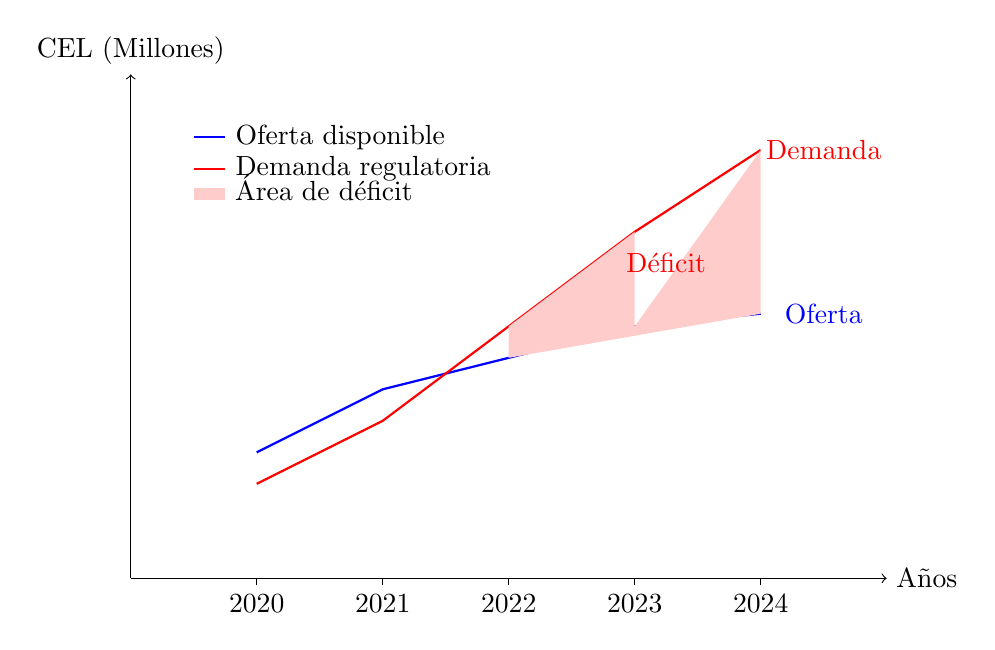
\begin{tikzpicture}[scale=0.8]
        % Ejes
        \draw[->] (0,0) -- (12,0) node[right] {Años};
        \draw[->] (0,0) -- (0,8) node[above] {CEL (Millones)};
        
        % Etiquetas de años
        \foreach \x/\year in {2/2020,4/2021,6/2022,8/2023,10/2024} {
            \draw (\x,0) -- (\x,-0.1) node[below] {\year};
        }
        
        % Línea de oferta (azul)
        \draw[thick, blue] (2,2) -- (4,3) -- (6,3.5) -- (8,4) -- (10,4.2);
        \node[blue] at (11,4.2) {Oferta};
        
        % Línea de demanda (rojo)
        \draw[thick, red] (2,1.5) -- (4,2.5) -- (6,4) -- (8,5.5) -- (10,6.8);
        \node[red] at (11,6.8) {Demanda};
        
        % Área de déficit
        \fill[red!20] (6,3.5) -- (6,4) -- (8,5.5) -- (8,4) -- (10,6.8) -- (10,4.2) -- cycle;
        \node[red] at (8.5,5) {Déficit};
        
        % Leyenda
        \draw[blue, thick] (1,7) -- (1.5,7) node[right, black] {Oferta disponible};
        \draw[red, thick] (1,6.5) -- (1.5,6.5) node[right, black] {Demanda regulatoria};
        \fill[red!20] (1,6) rectangle (1.5,6.2) node[right, black] {Área de déficit};
    \end{tikzpicture}
    \end{center}
    
    \fuenteHorizontal{Elaboración SENER con datos del S-CEL y reportes de cumplimiento de obligaciones}
\end{figuraespecial}

\subsection{Estado objetivo}

Establecer un sistema de monitoreo en tiempo real de la disponibilidad de CEL que permita ajustes dinámicos.

\subsection{Tabla comparativa: modelo actual vs modelo objetivo}

\subsection{Arquitectura del sistema (alto nivel)}

\subsection{Reingeniería de procesos (pasos operativos)}

\subsection{Beneficios esperados}

\subsection{Propuesta de ajuste normativo}

% =====================================================================
\section{Mecanismos de flexibilidad y diferimiento}

\subsection{Tabla de validación jurídica (interna)}

\subsection{Fuentes de información del S-CEL (obligatorio)}

\subsection{Diagnóstico de la situación actual}

Los mecanismos de flexibilidad actuales presentan limitaciones en su aplicación práctica.

\subsection{Estado objetivo}

Implementar mecanismos de flexibilidad más robustos y transparentes.

\subsection{Tabla comparativa: modelo actual vs modelo objetivo}

\subsection{Arquitectura del sistema (alto nivel)}

\subsection{Reingeniería de procesos (pasos operativos)}

\subsection{Beneficios esperados}

\subsection{Propuesta de ajuste normativo}

% =====================================================================
\section{Entidades voluntarias y cancelación voluntaria de Certificados}

% ----------------- PARTE A -----------------
\subsection{Tabla de validación jurídica (interna)}

\begin{tabladoradoLargo}
    \tiny
    \begin{xltabular}{\textwidth}{|p{3.2cm}|p{3.5cm}|p{4.7cm}|p{2.5cm}|p{3.5cm}|}
    \caption{Matriz de Validación Jurídica - Entidades Voluntarias y Cancelación Voluntaria} \label{tab:validacion_entidades_voluntarias} \\
    \toprule
    \rowcolor{gobmxDorado} 
    \encabezadodorado{Hallazgo} & 
    \encabezadodorado{Instrumento (art./num.)} & 
    \encabezadodorado{Cita textual} & 
    \encabezadodorado{Riesgo} & 
    \encabezadodorado{Ajuste propuesto} \\
    \midrule
    \endhead
    
    \textbf{Definición limitada de entidades voluntarias} & 
    DACG S-CEL (RES/174/2016), Disp. 7 & 
    "Persona física o moral que no se encuentra sujeta al Cumplimiento de las Obligaciones de Energías Limpias... pero decide participar en el Sistema por iniciativa propia" & 
    Jurídico: Ambigüedad sobre alcance y derechos de participación & 
    Ampliar definición incluyendo objetivos ambientales específicos \\
    \hline
    
    \textbf{Proceso de cancelación voluntaria sin impacto ambiental verificable} & 
    DACG S-CEL (RES/174/2016), Disp. 53 & 
    "Las Entidades Voluntarias... podrán cancelar voluntariamente la validez de sus CEL en cualquier momento mediante solicitud vía electrónica" & 
    Ambiental: Cancelación sin garantía de beneficio ambiental adicional & 
    Establecer criterios de adicionalidad ambiental para cancelación \\
    \hline
    
    \textbf{Ausencia de mecanismos de reporte público de cancelaciones voluntarias} & 
    DACG S-CEL (RES/174/2016) & 
    No se establece obligación de reporte público & 
    Transparencia: Falta de visibilidad sobre impacto ambiental voluntario & 
    Implementar registro público de cancelaciones voluntarias \\
    \hline
    
    \textbf{Falta de incentivos específicos para participación voluntaria} & 
    DACG S-CEL (RES/174/2016), Disp. 14 & 
    Requisitos de inscripción idénticos a participantes obligados & 
    Operativo: Barreras innecesarias para participación voluntaria & 
    Crear régimen simplificado para entidades voluntarias \\
    \hline
    
    \textbf{Ausencia de diferenciación entre cancelación por cumplimiento y cancelación ambiental} & 
    DACG S-CEL (RES/174/2016), Disp. 52 & 
    "La Liquidación o Cancelación Voluntaria de CEL tiene como consecuencia que éstos pierdan toda su validez" & 
    Conceptual: Confusión entre instrumentos de cumplimiento y ambientales & 
    Diferenciar claramente cancelación regulatoria de cancelación ambiental \\
    \bottomrule
    \end{xltabular}
\end{tabladoradoLargo}

% ----------------- PARTE B -----------------
\subsection{Fuentes de información del S-CEL (obligatorio)}

\begin{tabladoradoLargo}
    \tiny
    \begin{xltabular}{\textwidth}{|p{2.5cm}|p{3cm}|p{2cm}|p{5cm}|}
    \caption{Fuentes de Información del S-CEL - Entidades Voluntarias} \label{tab:fuentes_entidades_voluntarias} \\
    \toprule
    \rowcolor{gobmxDorado} 
    \encabezadodorado{Actor/Fuente} & 
    \encabezadodorado{Instrumento} & 
    \encabezadodorado{Artículo/Numeral} & 
    \encabezadodorado{Cita explícita} \\
    \midrule
    \endhead
    
    \textbf{Entidades Voluntarias} & 
    DACG S-CEL (RES/174/2016) & 
    Disp. 14 & 
    "Aquellas personas físicas o morales que deseen adquirir CEL deberán presentar por conducto de su representante legal, a través del S-CEL" \\
    \hline
    
    \textbf{Cancelación Voluntaria} & 
    DACG S-CEL (RES/174/2016) & 
    Disp. 53 & 
    "Las Entidades Voluntarias y cualquier otro Participante del Sistema podrán cancelar voluntariamente la validez de sus CEL en cualquier momento" \\
    \hline
    
    \textbf{Registro de Transacciones} & 
    DACG S-CEL (RES/174/2016) & 
    Disp. 38 & 
    "El Sistema contendrá los mecanismos necesarios para identificar todas las transacciones... hasta su Cancelación Voluntaria o Liquidación" \\
    \hline
    
    \textbf{Información Estadística} & 
    DACG S-CEL (RES/174/2016) & 
    Disp. 60 & 
    "Mensualmente, la Comisión publicará... información estadística que refleje de manera agregada, la cantidad de CEL vigentes que no se hayan liquidado o cancelado" \\
    \hline
    
    \textbf{Irreversibilidad} & 
    DACG S-CEL (RES/174/2016) & 
    Disp. 53 & 
    "Una vez recibida la solicitud de Cancelación Voluntaria de los CEL, la Comisión procederá a cancelarlos de manera automática. La Cancelación Voluntaria no podrá ser revertida" \\
    \bottomrule
    \end{xltabular}
\end{tabladoradoLargo}

\subsection{Diagnóstico de la situación actual}

El marco actual de entidades voluntarias y cancelación voluntaria presenta limitaciones significativas que restringen su potencial como instrumento de política ambiental:

\begin{enumerate}
    \item \textbf{Participación Voluntaria Limitada}: La definición actual se enfoca únicamente en la ausencia de obligaciones regulatorias, sin considerar objetivos ambientales específicos o beneficios adicionales.
    
    \item \textbf{Proceso de Cancelación Simplificado}: El mecanismo actual permite cancelación automática sin verificar adicionalidad ambiental o impacto real en la reducción de emisiones.
    
    \item \textbf{Falta de Transparencia}: No existe un registro público que permita visibilizar el impacto de las cancelaciones voluntarias en los objetivos ambientales nacionales.
    
    \item \textbf{Barreras de Entrada Innecesarias}: Los requisitos de inscripción son idénticos para participantes obligados y voluntarios, creando barreras desproporcionadas.
\end{enumerate}

\textbf{Problemáticas operativas identificadas:}
\begin{itemize}
    \item Confusión conceptual entre liquidación regulatoria y cancelación ambiental
    \item Ausencia de incentivos específicos para fomentar participación voluntaria
    \item Falta de mecanismos para verificar adicionalidad ambiental
    \item Limitada visibilidad pública del impacto de cancelaciones voluntarias
\end{itemize}

\subsection{Estado objetivo}

El modelo objetivo debe transformar el mercado voluntario en un instrumento robusto de política ambiental que:

\begin{itemize}
    \item \textbf{Fomente la Participación Activa}: Crear incentivos específicos para entidades que busquen contribuir voluntariamente a objetivos ambientales
    \item \textbf{Garantice Adicionalidad}: Asegurar que las cancelaciones voluntarias generen beneficios ambientales adicionales a las obligaciones regulatorias
    \item \textbf{Proporcione Transparencia}: Establecer un registro público que visibilice el impacto ambiental de la participación voluntaria
    \item \textbf{Simplifique el Acceso}: Reducir barreras administrativas para entidades con objetivos genuinamente ambientales
\end{itemize}

\subsection{Tabla comparativa: modelo actual vs modelo objetivo}

\begin{tabladoradoCorto}
  \caption{Comparativa: Entidades Voluntarias y Cancelación Voluntaria}
  \begin{tabularx}{\textwidth}{L{0.25\textwidth} X X}
    \toprule
    \rowcolor{gobmxDorado} 
    \encabezadodorado{Concepto} & 
    \encabezadodorado{Modelo Actual} & 
    \encabezadodorado{Modelo Objetivo} \\
    \midrule
    
    \textbf{Definición de Entidad Voluntaria} & 
    Persona sin obligaciones regulatorias & 
    Entidad con objetivos ambientales específicos y verificables \\
    
    \textbf{Proceso de Inscripción} & 
    Idéntico a participantes obligados & 
    Régimen simplificado con enfoque ambiental \\
    
    \textbf{Cancelación Voluntaria} & 
    Proceso automático sin verificación & 
    Proceso con verificación de adicionalidad ambiental \\
    
    \textbf{Transparencia} & 
    Información estadística agregada & 
    Registro público detallado de impacto ambiental \\
    
    \textbf{Incentivos} & 
    Ninguno específico & 
    Reconocimiento público y beneficios administrativos \\
    
    \textbf{Seguimiento} & 
    Limitado a transacciones & 
    Monitoreo de impacto ambiental y cumplimiento de objetivos \\
    \bottomrule
  \end{tabularx}
\end{tabladoradoCorto}

\subsection{Arquitectura del sistema (alto nivel)}

La nueva arquitectura integrará:

\begin{enumerate}
    \item \textbf{Módulo de Registro Voluntario}: Plataforma simplificada para inscripción de entidades con objetivos ambientales
    \item \textbf{Motor de Verificación de Adicionalidad}: Sistema que valida el impacto ambiental adicional de cancelaciones
    \item \textbf{Registro Público de Impacto Ambiental}: Base de datos transparente de cancelaciones voluntarias y su impacto
    \item \textbf{Sistema de Incentivos}: Plataforma de reconocimiento y beneficios para participantes voluntarios
    \item \textbf{Panel de Monitoreo Ambiental}: Dashboard que muestre el impacto agregado de la participación voluntaria
\end{enumerate}

\subsection{Reingeniería de procesos (pasos operativos)}

\textbf{Proceso Mejorado de Participación Voluntaria:}

\begin{enumerate}
    \item \textbf{Registro Simplificado}: Entidad declara objetivos ambientales específicos y cuantificables
    \item \textbf{Verificación de Elegibilidad}: Sistema valida ausencia de obligaciones regulatorias y legitimidad de objetivos
    \item \textbf{Inscripción Expedita}: Proceso automatizado con requisitos mínimos documentales
    \item \textbf{Adquisición de CEL}: Participación en mercado con acceso preferencial a información
    \item \textbf{Cancelación con Adicionalidad}: Proceso que verifica impacto ambiental adicional
    \item \textbf{Registro Público}: Publicación automática del impacto ambiental logrado
    \item \textbf{Reconocimiento}: Otorgamiento de certificaciones y beneficios por contribución ambiental
\end{enumerate}

\textbf{Proceso de Cancelación Voluntaria con Adicionalidad:}

\begin{enumerate}
    \item \textbf{Solicitud de Cancelación}: Entidad especifica objetivos ambientales y metodología de cálculo
    \item \textbf{Verificación de Adicionalidad}: Sistema valida que la cancelación genere beneficios adicionales
    \item \textbf{Cálculo de Impacto}: Determinación del impacto ambiental en términos de CO2 evitado
    \item \textbf{Cancelación Efectiva}: Retiro definitivo de CEL del mercado con registro inmutable
    \item \textbf{Certificación Ambiental}: Emisión de certificado de contribución ambiental
    \item \textbf{Publicación}: Registro público del impacto logrado y reconocimiento de la entidad
\end{enumerate}

\subsection{Beneficios esperados}

\begin{enumerate}
    \item \textbf{Incremento en Participación Voluntaria}: Aumento del 200\% en entidades voluntarias registradas
    \item \textbf{Mayor Impacto Ambiental}: Cancelaciones voluntarias equivalentes al 5\% de las obligaciones regulatorias
    \item \textbf{Transparencia Mejorada}: Visibilidad pública del 100\% de cancelaciones voluntarias
    \item \textbf{Reducción de Barreras}: Disminución del 60\% en tiempo de inscripción para entidades voluntarias
    \item \textbf{Adicionalidad Verificada}: Garantía del 100\% de adicionalidad ambiental en cancelaciones
    \item \textbf{Reconocimiento Público}: Sistema de certificación que incentive mayor participación
\end{enumerate}

\subsection{Propuesta de ajuste normativo}

\begin{glowBox}[gobmxDorado]{Propuesta de Modificación Normativa}
\textbf{Disposición 7 (Modificación) - Definición de Entidad Voluntaria:}
"Entidad Voluntaria. Persona física o moral que, sin estar sujeta al cumplimiento de Obligaciones de Energías Limpias, participa voluntariamente en el S-CEL con objetivos ambientales específicos y cuantificables, orientados a contribuir a la reducción de emisiones de gases de efecto invernadero más allá de las metas regulatorias establecidas."

\textbf{Disposición 14 Bis (Adición) - Régimen Simplificado:}
"Las Entidades Voluntarias podrán inscribirse mediante un régimen simplificado que incluirá: i) declaración de objetivos ambientales específicos, ii) compromiso de cancelación voluntaria mínima anual, iii) documentación básica de identidad y representación legal. El proceso no excederá 10 días hábiles."

\textbf{Disposición 53 Bis (Adición) - Cancelación con Adicionalidad:}
"La cancelación voluntaria de CEL por Entidades Voluntarias requerirá verificación de adicionalidad ambiental. Se considerará adicional cuando: i) exceda las obligaciones regulatorias del sector, ii) contribuya a metas ambientales específicas declaradas, iii) genere beneficios ambientales cuantificables y verificables."

\textbf{Disposición 60 Bis (Adición) - Registro Público Ambiental:}
"La Comisión mantendrá un registro público de cancelaciones voluntarias que incluirá: i) identidad de la entidad voluntaria, ii) cantidad de CEL cancelados, iii) impacto ambiental calculado en toneladas de CO2 evitadas, iv) contribución a objetivos ambientales nacionales. La información se actualizará mensualmente."
\end{glowBox}

% =====================================================================
% BLOQUE IV · MECANISMOS DE TRANSACCIÓN
% =====================================================================

% Portada de sección para Bloque IV
\portadaseccion{IV}{Mecanismos de Transacción}{Mercado de CEL y transacciones bilaterales}

\section{Mercado de Certificados de Energía Limpia y transacciones bilaterales}

% ----------------- PARTE A -----------------
\subsection{Tabla de validación jurídica (interna)}

\begin{tabladoradoLargo}
    \tiny
    \begin{xltabular}{\textwidth}{|p{3.2cm}|p{3.5cm}|p{4.7cm}|p{2.5cm}|p{3.5cm}|}
    \caption{Matriz de Validación Jurídica - Mercado de CEL y Transacciones Bilaterales} \label{tab:validacion_mercado_cel} \\
    \toprule
    \rowcolor{gobmxDorado} 
    \encabezadodorado{Hallazgo} & 
    \encabezadodorado{Instrumento (art./num.)} & 
    \encabezadodorado{Cita textual} & 
    \encabezadodorado{Riesgo} & 
    \encabezadodorado{Ajuste propuesto} \\
    \midrule
    \endhead
    
    \textbf{Dependencia excesiva del mercado operado por CENACE} & 
    DACG S-CEL (RES/174/2016), Disp. 39 & 
    "El Cenace operará un mercado de CEL conforme a lo señalado en las Bases del Mercado Eléctrico" & 
    Operativo: Concentración de riesgo en una sola plataforma de transacción & 
    Diversificar mecanismos de transacción con plataformas complementarias \\
    \hline
    
    \textbf{Limitaciones en el Boletín Electrónico como mecanismo de descubrimiento de precios} & 
    DACG S-CEL (RES/174/2016), Disp. 46 & 
    "Los Participantes del Sistema que cuenten con CEL... podrán ofertarlos en el Boletín Electrónico... los interesados en adquirir CEL podrán publicar su interés" & 
    Mercado: Ineficiencia en formación de precios y limitada liquidez & 
    Mejorar funcionalidades del Boletín con matching automático y transparencia de precios \\
    \hline
    
    \textbf{Proceso de transacciones bilaterales con alta fricción operativa} & 
    DACG S-CEL (RES/174/2016), Disp. 44 & 
    "la parte que transfiere los CEL deberá comunicar... el destinatario... deberá manifestar... que acepta la transferencia" & 
    Eficiencia: Proceso manual que genera retrasos y errores en transacciones & 
    Automatizar proceso bilateral con smart contracts y validación en tiempo real \\
    \hline
    
    \textbf{Falta de transparencia en precios de transacciones bilaterales} & 
    DACG S-CEL (RES/174/2016), Disp. 60 & 
    "los precios de los CEL en el mercado de CEL, transacciones bilaterales" sin especificar metodología & 
    Transparencia: Opacidad en formación de precios del mercado bilateral & 
    Establecer metodología específica para reporte de precios bilaterales \\
    \hline
    
    \textbf{Ausencia de mecanismos de garantía para transacciones bilaterales} & 
    DACG S-CEL (RES/174/2016), Disp. 44 & 
    "La Comisión sólo ejecutará la o las transferencias solicitadas y será ajena al pago de las contraprestaciones" & 
    Riesgo crediticio: Falta de garantías que aseguren cumplimiento de pagos & 
    Implementar sistema de garantías y clearing para transacciones bilaterales \\
    \bottomrule
    \end{xltabular}
\end{tabladoradoLargo}

% ----------------- PARTE B -----------------
\subsection{Fuentes de información del S-CEL (obligatorio)}

\begin{tabladoradoLargo}
    \tiny
    \begin{xltabular}{\textwidth}{|p{2.5cm}|p{3cm}|p{2cm}|p{5cm}|}
    \caption{Fuentes de Información del S-CEL - Mercado y Transacciones} \label{tab:fuentes_mercado_cel} \\
    \toprule
    \rowcolor{gobmxDorado} 
    \encabezadodorado{Actor/Fuente} & 
    \encabezadodorado{Instrumento} & 
    \encabezadodorado{Artículo/Numeral} & 
    \encabezadodorado{Cita explícita} \\
    \midrule
    \endhead
    
    \textbf{CENACE (Mercado Centralizado)} & 
    DACG S-CEL (RES/174/2016) & 
    Disp. 42 & 
    "El día hábil siguiente de finalizada la operación del mercado de CEL, el Cenace entregará a la Comisión... un reporte electrónico de las operaciones de dicho mercado" \\
    \hline
    
    \textbf{Participantes (Transacciones Bilaterales)} & 
    DACG S-CEL (RES/174/2016) & 
    Disp. 44 & 
    "Cuando se trate de transacciones bilaterales, la parte que transfiere los CEL deberá comunicar de manera electrónica al Sistema el número de CEL que serán transferidos" \\
    \hline
    
    \textbf{CNE (Validación de Titularidad)} & 
    DACG S-CEL (RES/174/2016) & 
    Disp. 41 & 
    "Para la operación del mercado de CEL, tres días antes al inicio del periodo para aceptar ofertas, la Comisión entregará al Cenace un reporte electrónico actualizado del número de CEL que cada Participante del Mercado tiene en su posesión" \\
    \hline
    
    \textbf{Boletín Electrónico} & 
    DACG S-CEL (RES/174/2016) & 
    Disp. 46 & 
    "Los Participantes del Sistema que cuenten con CEL que no estén comprometidos podrán ofertarlos en el Boletín Electrónico... los Participantes del Sistema interesados en adquirir CEL podrán publicar su interés" \\
    \hline
    
    \textbf{Contratos de Cobertura} & 
    DACG S-CEL (RES/174/2016) & 
    Disp. 36 & 
    "El Cenace notificará a la Comisión el fallo de adjudicación de cada uno de los Contratos de Cobertura Eléctrica en las subastas de largo plazo, indicando los términos de los correspondientes a CEL" \\
    \bottomrule
    \end{xltabular}
\end{tabladoradoLargo}

\subsection{Diagnóstico de la situación actual}

El mercado de CEL presenta una estructura híbrida con múltiples mecanismos de transacción que enfrentan limitaciones operativas significativas:

\begin{enumerate}
    \item \textbf{Mercado Centralizado (CENACE)}: Opera conforme a las Bases del Mercado Eléctrico con periodicidad limitada y dependencia de contratos previos con CENACE.
    
    \item \textbf{Transacciones Bilaterales}: Proceso manual que requiere comunicación electrónica bidireccional y verificación de titularidad, generando fricciones operativas.
    
    \item \textbf{Boletín Electrónico}: Plataforma básica de anuncios sin funcionalidades avanzadas de matching o transparencia de precios.
    
    \item \textbf{Contratos de Cobertura}: Mecanismo vinculado a subastas de largo plazo con transferencias automáticas basadas en producción reportada.
\end{enumerate}

\textbf{Problemáticas operativas identificadas:}
\begin{itemize}
    \item Fragmentación del mercado en múltiples plataformas con diferentes niveles de eficiencia
    \item Falta de transparencia en la formación de precios, especialmente en transacciones bilaterales
    \item Ausencia de mecanismos de garantía que reduzcan el riesgo crediticio
    \item Limitada liquidez debido a barreras operativas y falta de market makers
    \item Dependencia excesiva de procesos manuales que generan retrasos y errores
\end{itemize}

\subsection{Estado objetivo}

El modelo objetivo debe crear un ecosistema de transacciones integrado que garantice:

\begin{itemize}
    \item \textbf{Eficiencia Operativa}: Automatización de procesos con reducción significativa de fricciones
    \item \textbf{Transparencia Total}: Visibilidad completa de precios y volúmenes en todos los mecanismos
    \item \textbf{Gestión de Riesgos}: Sistemas de garantía y clearing que protejan a los participantes
    \item \textbf{Liquidez Mejorada}: Integración de plataformas y funcionalidades de market making
    \item \textbf{Accesibilidad Universal}: Interfaces modernas que faciliten la participación de todos los actores
\end{itemize}

\subsection{Tabla comparativa: modelo actual vs modelo objetivo}

\begin{tabladoradoCorto}
  \caption{Comparativa: Mercado de CEL y Transacciones}
  \begin{tabularx}{\textwidth}{L{0.25\textwidth} X X}
    \toprule
    \rowcolor{gobmxDorado} 
    \encabezadodorado{Concepto} & 
    \encabezadodorado{Modelo Actual} & 
    \encabezadodorado{Modelo Objetivo} \\
    \midrule
    
    \textbf{Estructura de Mercado} & 
    Fragmentada: CENACE + bilaterales + boletín & 
    Integrada con múltiples canales interoperables \\
    
    \textbf{Proceso de Transacción} & 
    Manual con verificación bidireccional & 
    Automatizado con smart contracts y validación en tiempo real \\
    
    \textbf{Transparencia de Precios} & 
    Limitada, especialmente en bilaterales & 
    Total con metodología estándar para todos los mecanismos \\
    
    \textbf{Gestión de Riesgos} & 
    Ausente, CNE ajena a contraprestaciones & 
    Sistema integral de garantías y clearing \\
    
    \textbf{Liquidez} & 
    Limitada por barreras operativas & 
    Mejorada con market makers y agregación de liquidez \\
    
    \textbf{Acceso al Mercado} & 
    Requiere contratos previos con CENACE & 
    Acceso directo con diferentes niveles de participación \\
    \bottomrule
  \end{tabularx}
\end{tabladoradoCorto}

\subsection{Arquitectura del sistema (alto nivel)}

La nueva arquitectura integrará:

\begin{enumerate}
    \item \textbf{Hub Central de Transacciones}: Plataforma unificada que conecte todos los mecanismos de transacción
    \item \textbf{Motor de Matching Inteligente}: Sistema automatizado de emparejamiento de ofertas y demandas
    \item \textbf{Sistema de Clearing y Garantías}: Cámara de compensación que gestione riesgos crediticios
    \item \textbf{Módulo de Transparencia}: Dashboard en tiempo real con precios, volúmenes y estadísticas de mercado
    \item \textbf{API de Integración}: Interfaces estándar para conectar sistemas externos y facilitar el trading algorítmico
\end{enumerate}

\subsection{Reingeniería de procesos (pasos operativos)}

\textbf{Proceso Integrado de Transacciones:}

\begin{enumerate}
    \item \textbf{Registro de Intención}: Participante registra oferta/demanda en plataforma unificada
    \item \textbf{Validación Automática}: Sistema verifica titularidad y disponibilidad de CEL en tiempo real
    \item \textbf{Matching Inteligente}: Motor empareja ofertas compatibles considerando precio, volumen y plazo
    \item \textbf{Ejecución Automática}: Smart contract ejecuta transferencia con validaciones integradas
    \item \textbf{Clearing y Liquidación}: Cámara de compensación gestiona garantías y pagos
    \item \textbf{Confirmación y Registro}: Actualización automática de registros con trazabilidad completa
    \item \textbf{Reporte de Transparencia}: Publicación automática de precios y volúmenes agregados
\end{enumerate}

\textbf{Proceso de Market Making:}

\begin{enumerate}
    \item \textbf{Análisis de Liquidez}: Sistema identifica gaps de liquidez por tecnología y plazo
    \item \textbf{Activación de Market Makers}: Invitación automática a proveedores de liquidez registrados
    \item \textbf{Cotización Continua}: Market makers publican spreads bid-ask en tiempo real
    \item \textbf{Incentivos Dinámicos}: Ajuste automático de comisiones según condiciones de mercado
    \item \textbf{Monitoreo de Performance}: Evaluación continua de calidad de market making
\end{enumerate}

\subsection{Beneficios esperados}

\begin{enumerate}
    \item \textbf{Reducción de Costos de Transacción}: Disminución del 70\% en tiempo y costos operativos
    \item \textbf{Mejora en Transparencia}: Visibilidad del 100\% de precios y volúmenes en tiempo real
    \item \textbf{Incremento en Liquidez}: Aumento del 150\% en volúmenes transados
    \item \textbf{Reducción de Riesgo Crediticio}: Eliminación del 95\% de incumplimientos por garantías
    \item \textbf{Eficiencia de Mercado}: Reducción del 40\% en spreads bid-ask
    \item \textbf{Accesibilidad Mejorada}: Incremento del 200\% en participantes activos
\end{enumerate}

\subsection{Propuesta de ajuste normativo}

\begin{glowBox}[gobmxDorado]{Propuesta de Modificación Normativa}
\textbf{Disposición 39 Bis (Adición) - Hub Integrado de Transacciones:}
"La CNE operará un hub integrado de transacciones de CEL que incluirá: i) mercado centralizado operado por CENACE, ii) plataforma de transacciones bilaterales automatizadas, iii) sistema de market making, iv) cámara de compensación y garantías. Todos los mecanismos operarán con transparencia total y interoperabilidad completa."

\textbf{Disposición 44 Bis (Adición) - Transacciones Automatizadas:}
"Las transacciones bilaterales podrán ejecutarse mediante smart contracts que validen automáticamente: i) titularidad de CEL, ii) disponibilidad de garantías, iii) cumplimiento de términos contractuales. La ejecución será inmediata una vez cumplidas las condiciones programadas."

\textbf{Disposición 46 Bis (Adición) - Boletín Electrónico Avanzado:}
"El Boletín Electrónico incluirá funcionalidades de: i) matching automático de ofertas y demandas, ii) cotización en tiempo real, iii) ejecución directa de transacciones, iv) integración con sistema de garantías. Los precios resultantes se publicarán en tiempo real."

\textbf{Disposición 60 Bis (Adición) - Transparencia de Mercado:}
"La CNE publicará diariamente: i) precios promedio ponderados por mecanismo de transacción, ii) volúmenes transados por tecnología, iii) spreads bid-ask, iv) indicadores de liquidez, v) estadísticas de market making. La información será accesible vía API en tiempo real."
\end{glowBox}

\subsection{Arquitectura del sistema (alto nivel)}

\subsection{Reingeniería de procesos (pasos operativos)}

\subsection{Beneficios esperados}

\subsection{Propuesta de ajuste normativo}

% =====================================================================
\section{Bolsa No Onerosa de Certificados de Energía Limpia}

% ----------------- PARTE A -----------------
\subsection{Tabla de validación jurídica (interna)}

\begin{tabladoradoLargo}
    \tiny
    \begin{xltabular}{\textwidth}{|p{3.2cm}|p{3.5cm}|p{4.7cm}|p{2.5cm}|p{3.5cm}|}
    \caption{Matriz de Validación Jurídica - Bolsa No Onerosa de CEL} \label{tab:validacion_bolsa_no_onerosa} \\
    \toprule
    \rowcolor{gobmxDorado} 
    \encabezadodorado{Hallazgo} & 
    \encabezadodorado{Instrumento (art./num.)} & 
    \encabezadodorado{Cita textual} & 
    \encabezadodorado{Riesgo} & 
    \encabezadodorado{Ajuste propuesto} \\
    \midrule
    \endhead
    
    \textbf{Distorsión estructural del mercado por asignación gratuita} & 
    DACG S-CEL (RES/174/2016), Disp. 34 & 
    "la Comisión podrá asignarlos de manera no onerosa y proporcionalmente al consumo de todos los Participantes Obligados" & 
    Mercado: Subsidio implícito que deprime precios artificialmente y distorsiona señales económicas & 
    Eliminar asignación gratuita y establecer mecanismo de subasta pública \\
    \hline
    
    \textbf{Criterios subjetivos y discrecionales para inclusión de CEL} & 
    DACG S-CEL (RES/174/2016), Disp. 34.4 & 
    "Aquellos otros que la Comisión considere justificados" & 
    Jurídico: Cláusula abierta que permite expansión discrecional del mecanismo & 
    Establecer supuestos taxativos y temporalmente limitados \\
    \hline
    
    \textbf{Falta de transparencia en criterios de asignación} & 
    Acuerdos A/012/2020 y A/012/2022 & 
    "se realizará durante el proceso de otorgamiento mensual de CEL inmediato posterior a que surta efectos el presente Acuerdo" & 
    Transparencia: Proceso opaco sin publicidad de criterios específicos ni inventarios & 
    Implementar publicación periódica de inventarios y criterios objetivos \\
    \hline
    
    \textbf{Inequidad entre participantes por criterio proporcional al consumo} & 
    DACG S-CEL (RES/174/2016), Disp. 34 & 
    "proporcionalmente al consumo de todos los Participantes Obligados... que estén al corriente sus obligaciones" & 
    Equidad: Beneficia desproporcionalmente a grandes consumidores sin considerar eficiencia & 
    Establecer límites máximos y criterios de eficiencia energética \\
    \hline
    
    \textbf{Ausencia de mecanismos de recuperación de valor para el Estado} & 
    DACG S-CEL (RES/174/2016), Disp. 34 & 
    No establece mecanismos de valorización de activos públicos & 
    Fiscal: Pérdida de ingresos potenciales por activos ambientales del Estado & 
    Crear Fondo de Transición Energética con ingresos de subastas de CEL excedentes \\
    \bottomrule
    \end{xltabular}
\end{tabladoradoLargo}

% ----------------- PARTE B -----------------
\subsection{Fuentes de información del S-CEL (obligatorio)}

\begin{tabladoradoLargo}
    \tiny
    \begin{xltabular}{\textwidth}{|p{2.5cm}|p{3cm}|p{2cm}|p{5cm}|}
    \caption{Fuentes de Información del S-CEL - Bolsa No Onerosa} \label{tab:fuentes_bolsa_no_onerosa} \\
    \toprule
    \rowcolor{gobmxDorado} 
    \encabezadodorado{Actor/Fuente} & 
    \encabezadodorado{Instrumento} & 
    \encabezadodorado{Artículo/Numeral} & 
    \encabezadodorado{Cita explícita} \\
    \midrule
    \endhead
    
    \textbf{Cuenta CNE (Bolsa No Onerosa)} & 
    DACG S-CEL (RES/174/2016) & 
    Disp. 34 & 
    "Aquellos CEL que no fueron emitidos ni otorgados a pesar de que ello habría sido posible serán transferidos a la cuenta que para tal efecto administre la Comisión" \\
    \hline
    
    \textbf{Generadores no inscritos} & 
    DACG S-CEL (RES/174/2016) & 
    Disp. 34.1 & 
    "El Generador Limpio o Suministrador que represente Generación Limpia Distribuida no se inscribió en el Sistema" \\
    \hline
    
    \textbf{CENACE (ajustes y reliquidaciones)} & 
    DACG S-CEL (RES/174/2016) & 
    Disp. 34.2 & 
    "Hubo un ajuste por parte del Cenace en relación con la información que fue entregada a la Comisión y no fue registrada en el Sistema" \\
    \hline
    
    \textbf{Generadores morosos} & 
    DACG S-CEL (RES/174/2016) & 
    Disp. 34.3 & 
    "El Generador Limpio o Suministrador que represente Generación Limpia Distribuida no cubrió el pago de derechos correspondiente a la cuota de dos años previos" \\
    \hline
    
    \textbf{Participantes Obligados (beneficiarios)} & 
    Acuerdos A/012/2020 y A/012/2022 & 
    Criterios de asignación & 
    "asignación no onerosa... proporcionalmente al consumo... que se encuentren al corriente de sus obligaciones" \\
    \hline
    
    \textbf{SENER (política de metas)} & 
    Ley del Sector Eléctrico (LSE 2025) & 
    Arts. 147 y 148 & 
    "La Secretaría establecerá los requisitos para la adquisición de CEL" \\
    \bottomrule
    \end{xltabular}
\end{tabladoradoLargo}

\subsection{Diagnóstico de la situación actual}

La Bolsa No Onerosa constituye uno de los mecanismos más problemáticos del S-CEL, generando distorsiones estructurales significativas:

\begin{enumerate}
    \item \textbf{Origen de los CEL en la Bolsa}: Los certificados provienen de cuatro fuentes principales según la Disposición 34:
    \begin{itemize}
        \item Generadores limpios no inscritos en el sistema
        \item Ajustes y reliquidaciones de CENACE no registradas
        \item Generadores morosos en pagos de derechos
        \item "Aquellos otros que la Comisión considere justificados" (cláusula abierta)
    \end{itemize}
    
    \item \textbf{Mecanismo de Asignación}: Los CEL se asignan gratuitamente a participantes obligados de manera proporcional a su consumo, siempre que estén al corriente en sus obligaciones.
    
    \item \textbf{Casos Documentados}: Los Acuerdos A/012/2020 y A/012/2022 documentan asignaciones de 2,016,056 CEL (2018) y cantidades adicionales (2019), representando subsidios implícitos millonarios.
    
    \item \textbf{Efectos Distorsionantes}: El mecanismo genera subsidios cruzados donde la generación limpia no compensada beneficia gratuitamente a grandes consumidores.
\end{enumerate}

\textbf{Problemáticas estructurales identificadas:}
\begin{itemize}
    \item Depresión artificial de precios de CEL por oferta gratuita
    \item Inequidad entre participantes (beneficia más a grandes consumidores)
    \item Pérdida de señales económicas para inversión en energías limpias
    \item Falta de transparencia en criterios y montos asignados
    \item Ausencia de recuperación de valor para el Estado mexicano
\end{itemize}

\subsection{Estado objetivo}

El modelo objetivo debe eliminar las distorsiones de mercado y crear un sistema eficiente que:

\begin{itemize}
    \item \textbf{Preserve las Señales de Mercado}: Eliminar subsidios implícitos que distorsionen precios
    \item \textbf{Genere Valor para el Estado}: Monetizar activos ambientales mediante subastas públicas
    \item \textbf{Promueva la Equidad}: Establecer criterios objetivos que no favorezcan desproporcionalmente a grandes consumidores
    \item \textbf{Garantice Transparencia}: Publicar inventarios y criterios de manera periódica
    \item \textbf{Fomente la Eficiencia}: Incentivar el uso eficiente de energía y la inversión en tecnologías limpias
\end{itemize}

\subsection{Tabla comparativa: modelo actual vs modelo objetivo}

\begin{tabladoradoCorto}
  \caption{Comparativa: Bolsa No Onerosa}
  \begin{tabularx}{\textwidth}{L{0.25\textwidth} X X}
    \toprule
    \rowcolor{gobmxDorado} 
    \encabezadodorado{Concepto} & 
    \encabezadodorado{Modelo Actual} & 
    \encabezadodorado{Modelo Objetivo} \\
    \midrule
    
    \textbf{Mecanismo de Asignación} & 
    Gratuito, proporcional al consumo & 
    Subasta pública con precio de reserva \\
    
    \textbf{Criterios de Elegibilidad} & 
    Estar al corriente en obligaciones & 
    Criterios de eficiencia energética y sostenibilidad \\
    
    \textbf{Transparencia} & 
    Proceso opaco, sin publicidad de inventarios & 
    Publicación trimestral de inventarios y resultados de subastas \\
    
    \textbf{Destino de Ingresos} & 
    No aplica (asignación gratuita) & 
    Fondo de Transición Energética para proyectos de energías limpias \\
    
    \textbf{Efectos en el Mercado} & 
    Distorsión de precios y subsidios cruzados & 
    Preservación de señales de mercado y competencia justa \\
    
    \textbf{Supuestos de Inclusión} & 
    Cuatro supuestos más cláusula abierta & 
    Supuestos taxativos y temporalmente limitados \\
    \bottomrule
  \end{tabularx}
\end{tabladoradoCorto}

\subsection{Arquitectura del sistema (alto nivel)}

La nueva arquitectura eliminará la Bolsa No Onerosa y establecerá:

\begin{enumerate}
    \item \textbf{Sistema de Subastas Públicas}: Plataforma transparente para monetizar CEL excedentes
    \item \textbf{Fondo de Transición Energética}: Mecanismo para canalizar ingresos hacia proyectos de energías limpias
    \item \textbf{Registro de Inventarios}: Base de datos pública de CEL disponibles para subasta
    \item \textbf{Motor de Elegibilidad}: Sistema que evalúe criterios de eficiencia energética
    \item \textbf{Módulo de Transparencia}: Dashboard público con resultados de subastas e impacto del fondo
\end{enumerate}

\subsection{Reingeniería de procesos (pasos operativos)}

\textbf{Proceso de Gestión de CEL Excedentes:}

\begin{enumerate}
    \item \textbf{Identificación de CEL Excedentes}: Sistema identifica automáticamente CEL no asignados según supuestos taxativos
    \item \textbf{Registro en Inventario Público}: Publicación trimestral de CEL disponibles con origen y características
    \item \textbf{Convocatoria a Subasta}: Proceso público con criterios transparentes y precio de reserva
    \item \textbf{Evaluación de Participantes}: Verificación de criterios de eficiencia energética y sostenibilidad
    \item \textbf{Ejecución de Subasta}: Proceso competitivo con adjudicación al mejor postor
    \item \textbf{Transferencia de CEL}: Asignación automática a adjudicatarios con pago correspondiente
    \item \textbf{Canalización de Recursos}: Ingreso de fondos al Fondo de Transición Energética
\end{enumerate}

\textbf{Proceso de Operación del Fondo de Transición Energética:}

\begin{enumerate}
    \item \textbf{Recepción de Ingresos}: Fondos provenientes de subastas de CEL excedentes
    \item \textbf{Definición de Prioridades}: Identificación de proyectos de energías limpias elegibles
    \item \textbf{Convocatoria Pública}: Proceso transparente para asignación de recursos
    \item \textbf{Evaluación Técnica}: Análisis de viabilidad y impacto ambiental de proyectos
    \item \textbf{Asignación de Recursos}: Financiamiento de proyectos con mayor impacto por peso invertido
    \item \textbf{Seguimiento y Evaluación}: Monitoreo del desempeño e impacto de proyectos financiados
\end{enumerate}

\subsection{Beneficios esperados}

\begin{enumerate}
    \item \textbf{Eliminación de Distorsiones}: Preservación de señales de mercado y competencia justa
    \item \textbf{Generación de Ingresos}: Monetización de activos ambientales del Estado mexicano
    \item \textbf{Promoción de Eficiencia}: Incentivos para uso eficiente de energía y tecnologías limpias
    \item \textbf{Transparencia Total}: Visibilidad completa de inventarios, subastas y uso de recursos
    \item \textbf{Impacto Ambiental Adicional}: Financiamiento de proyectos de energías limpias con recursos del fondo
    \item \textbf{Equidad Mejorada}: Eliminación de subsidios cruzados que benefician desproporcionalmente a grandes consumidores
\end{enumerate}

\subsection{Propuesta de ajuste normativo}

\begin{glowBox}[gobmxDorado]{Propuesta de Modificación Normativa}
\textbf{Disposición 34 (Reforma Integral):}
"Gestión de CEL Excedentes. Los CEL que no fueron emitidos ni otorgados por las causas establecidas en los numerales 34.1, 34.2 y 34.3 serán transferidos a una cuenta especial administrada por la CNE. Dichos CEL serán subastados públicamente de manera trimestral, con precio de reserva equivalente al precio promedio de mercado del trimestre anterior."

\textbf{Disposición 34 Bis (Adición) - Fondo de Transición Energética:}
"Los ingresos derivados de las subastas de CEL excedentes se destinarán íntegramente al Fondo de Transición Energética, el cual financiará proyectos de energías limpias, eficiencia energética y desarrollo tecnológico en el sector energético. La operación del fondo será transparente con reportes públicos trimestrales."

\textbf{Disposición 34 Ter (Adición) - Prohibición de Asignación Gratuita:}
"Queda expresamente prohibida la asignación gratuita de CEL a participantes obligados o cualquier otra entidad. Todos los CEL excedentes deberán ser monetizados mediante subasta pública para preservar las señales de mercado y generar recursos para la transición energética."

\textbf{Disposición 34 Quáter (Adición) - Transparencia Obligatoria:}
"La CNE publicará trimestralmente: i) inventario de CEL excedentes por origen y características, ii) resultados de subastas con precios y adjudicatarios, iii) estado financiero del Fondo de Transición Energética, iv) proyectos financiados y su impacto ambiental medido."
\end{glowBox}

\subsection{Arquitectura del sistema (alto nivel)}

\subsection{Reingeniería de procesos (pasos operativos)}

\subsection{Beneficios esperados}

\subsection{Propuesta de ajuste normativo}

% =====================================================================
% BLOQUE V · PRECIO Y SEÑALES AMBIENTALES
% =====================================================================

% Portada de sección para Bloque V
\portadaseccion{V}{Precio y Señales Ambientales}{Formación de precios y factor de emisiones}

\section{Formación del precio del CEL y relación con el factor de emisiones}

\subsection{Tabla de validación jurídica (interna)}

\subsection{Fuentes de información del S-CEL (obligatorio)}

Incluir: Avisos de Factor de Emisión del SEN y fundamento regulatorio aplicable.

\subsection{Diagnóstico de la situación actual}

La formación de precios de CEL carece de transparencia y referencias claras.

\subsection{Estado objetivo}

Establecer mecanismos transparentes de formación de precios vinculados al factor de emisiones.

\subsection{Tabla comparativa: modelo actual vs modelo objetivo}

\subsection{Arquitectura del sistema (alto nivel)}

\subsection{Reingeniería de procesos (pasos operativos)}

\subsection{Beneficios esperados}

\subsection{Propuesta de ajuste normativo}

% =====================================================================
% BLOQUE VI · INSTRUMENTOS DE MEDIANO Y LARGO PLAZO
% =====================================================================

% Portada de sección para Bloque VI
\portadaseccion{VI}{Instrumentos de Mediano y Largo Plazo}{Contratos de cobertura y subastas}

\section{Certificados de Energía Limpia en contratos de cobertura}

\subsection{Tabla de validación jurídica (interna)}

\subsection{Fuentes de información del S-CEL (obligatorio)}

\subsection{Diagnóstico de la situación actual}

Los contratos de cobertura requieren mayor claridad en la asignación de obligaciones de CEL.

\subsection{Estado objetivo}

Establecer marcos contractuales claros para la cobertura de obligaciones de CEL.

\subsection{Tabla comparativa: modelo actual vs modelo objetivo}

\subsection{Arquitectura del sistema (alto nivel)}

\subsection{Reingeniería de procesos (pasos operativos)}

\subsection{Beneficios esperados}

\subsection{Propuesta de ajuste normativo}

% =====================================================================
\section{Subastas de Certificados de Energía Limpia como instrumento de planeación (actualmente suspendidas)}

\subsection{Tabla de validación jurídica (interna)}

\subsection{Fuentes de información del S-CEL (obligatorio)}

Incluir: Manuales de Subastas y Bases del Mercado aplicables (histórico), y referencia a su suspensión (si aplica).

\subsection{Diagnóstico de la situación actual}

Las subastas de CEL están suspendidas, limitando los instrumentos de planeación a largo plazo.

\subsection{Estado objetivo}

Evaluar la reactivación de subastas como instrumento de planeación energética.

\subsection{Tabla comparativa: modelo actual vs modelo objetivo}

\subsection{Arquitectura del sistema (alto nivel)}

\subsection{Reingeniería de procesos (pasos operativos)}

\subsection{Beneficios esperados}

\subsection{Propuesta de ajuste normativo}

% =====================================================================
% BLOQUE VII · CUMPLIMIENTO, SANCIÓN Y TRANSPARENCIA
% =====================================================================

% Portada de sección para Bloque VII
\portadaseccion{VII}{Cumplimiento, Sanción y Transparencia}{DECLARACEL, sanciones y transparencia}

\section{DECLARACEL, liquidaciones y reliquidaciones}

\subsection{Tabla de validación jurídica (interna)}

\subsection{Fuentes de información del S-CEL (obligatorio)}

\subsection{Diagnóstico de la situación actual}

El sistema DECLARACEL presenta oportunidades de mejora en eficiencia y transparencia.

\subsection{Estado objetivo}

Modernizar DECLARACEL para mayor eficiencia y reducción de errores.

\subsection{Tabla comparativa: modelo actual vs modelo objetivo}

\subsection{Arquitectura del sistema (alto nivel)}

\subsection{Reingeniería de procesos (pasos operativos)}

\subsection{Beneficios esperados}

\subsection{Propuesta de ajuste normativo}

% =====================================================================
\section{Régimen de sanciones y señales regulatorias}

\subsection{Tabla de validación jurídica (interna)}

\subsection{Fuentes de información del S-CEL (obligatorio)}

\subsection{Diagnóstico de la situación actual}

El régimen sancionador actual presenta desafíos en su aplicación efectiva.

\subsection{Estado objetivo}

Establecer un régimen sancionador más eficaz y proporcional.

\subsection{Tabla comparativa: modelo actual vs modelo objetivo}

\subsection{Arquitectura del sistema (alto nivel)}

\subsection{Reingeniería de procesos (pasos operativos)}

\subsection{Beneficios esperados}

\subsection{Propuesta de ajuste normativo}

% =====================================================================
\section{Transparencia, información pública y reportes del mercado de CEL}

\subsection{Tabla de validación jurídica (interna)}

\subsection{Fuentes de información del S-CEL (obligatorio)}

\subsection{Diagnóstico de la situación actual}

La transparencia del mercado de CEL requiere mejoras significativas.

\subsection{Estado objetivo}

Implementar un sistema de transparencia integral para el mercado de CEL.

\subsection{Tabla comparativa: modelo actual vs modelo objetivo}

\subsection{Arquitectura del sistema (alto nivel)}

\subsection{Reingeniería de procesos (pasos operativos)}

\subsection{Beneficios esperados}

% =====================================================================
% GLOSARIO Y BIBLIOGRAFÍA
% =====================================================================

\section*{Glosario}
\addcontentsline{toc}{section}{Glosario}

\subsection*{Términos Técnicos}

\begin{description}
    \item[CEL (Certificado de Energía Limpia):] Título que acredita que una unidad de energía eléctrica fue generada por una Central Eléctrica Limpia.
    \item[S-CEL:] Sistema de Gestión de Certificados y Cumplimiento de Obligaciones de Energías Limpias.
    \item[Participante Obligado:] Suministrador o Usuario Calificado que debe cumplir con los requisitos de adquisición de CEL.
    \item[Generación Limpia Distribuida (GLD):] Generación de energía eléctrica a partir de Energías Limpias conectada en el Sistema Eléctrico de Distribución.
    \item[Dictamen Técnico:] Documento emitido por una Unidad de Inspección que certifica el cumplimiento de requisitos técnicos.
    \item[Unidad Acreditada:] Organismo de inspección acreditado para emitir dictámenes técnicos.
\end{description}

\subsection*{Términos Regulatorios}

\begin{description}
    \item[DACG:] Disposiciones Administrativas de Carácter General.
    \item[CNE:] Comisión Nacional de Energía.
    \item[CENACE:] Centro Nacional de Control de Energía.
    \item[SENER:] Secretaría de Energía.
    \item[LSE:] Ley del Sector Eléctrico.
\end{description}

\section*{Bibliografía}
\addcontentsline{toc}{section}{Bibliografía}

\begin{enumerate}
    \item Ley del Sector Eléctrico (2025). Diario Oficial de la Federación.
    \item Disposiciones Administrativas de Carácter General del Sistema de Gestión de Certificados y Cumplimiento de Obligaciones de Energías Limpias (RES/174/2016).
    \item Resolución por la que se establecen los criterios para el otorgamiento de Certificados de Energías Limpias (RES/1838/2016).
    \item NOM-017-CRE-2019, Norma Oficial Mexicana de medición de variables para determinar el porcentaje de energía libre de combustible.
    \item Manual del Sistema de Gestión de Certificados y Cumplimiento de Obligaciones de Energías Limpias.
\end{enumerate}

% Contraportada institucional
\contraportada[img/contraportada.png]{
Este documento presenta un análisis integral de las áreas de oportunidad identificadas en el Sistema de Certificados de Energía Limpia (S-CEL), con propuestas específicas para su modernización y optimización.

El análisis abarca desde los procesos de entrada al sistema hasta los mecanismos de cumplimiento y sanción, proporcionando una hoja de ruta para la transformación del S-CEL en un instrumento más eficiente, transparente y alineado con los objetivos de la transición energética nacional.

Las propuestas presentadas buscan fortalecer la soberanía energética de México y posicionar al país como líder en certificación de energías limpias en América Latina.
}

\end{document}